\section{Design for X}

\acf{DfX} concerns the development of guidelines and principles that support engineers in developing optimised products for a particular area. Examples include the Design for:

\begin{multicols}{2}
  \begin{itemize}
    \item Additive (3D Printing)
    \item Assembly
    \item Environment
    \item Disassembly
    \item Manufacturing
    \item Inspection
    \item Safety
    \item Service
    \item Six Sigma
  \end{itemize}
\end{multicols}


It is not uncommon for a products design to go through a number of iterations where the engineering design team will focus on a particular \ac{DfX} element. Over the course of the design, compromises will have to be made to develop a product that meets all these requirements.

In this exercise, we will focus on principles around \acf{DfA} and \acf{DfM}. Successful \ac{DfA} and \ac{DfM} activities will reduce the material, overhead and labour costs incurred when producing the product. Remember, 70-80\% of the committed cost is made at the design stage!\cite{ullman2002}\cite{corbett1986}\cite{mileham1993}

\acf{DfA}\marginnote{Design for Assembly} covers the principles and techniques that support the development of a design that is easy to assemble. Significant reductions in cost and the number of parts required to produce a product can be achieved through using these techniques.

Thus, \ac{DfA} is mainly concerned with minimising the number of assembly operations. This is often achieved by reducing the part count by combining part geometries together in order to increase their functionality. It is therefore common to see a decrease in parts and increase in part complexity after a \ac{DfA}  exercise is performed on a product. 

\acf{DfM}\marginnote{Design for Manufacture} covers the principles and guidelines that support designers in selecting an appropriate manufacturing technique for a component and optimising a components geometry for a particular technique. Optimising a design for manufacture can greatly reduce manufacturing lead-times and production costs. 

In this exercise, you will be using the tools available in the student workshops, rapid prototyping tools including laser cutting and 3D printing, and buying in standard components. The following sections will cover:

\begin{itemize}
  \item Design for (Manual) Assembly
  \item Design for Manufacture (Laser Cutting)
  \item Design for Manufacture (3D Printing)
\end{itemize}

Although we are focusing on laser cutting and 3D printing technologies in these course notes. You should also be looking back at your student workshop experience and bring that knowledge to bear on the development of the manufacturing processes for your components. So remember to think about the use of:

\begin{itemize}
  \item Hand-tools;
  \item Lathes;
  \item Pillar drills; and,
  \item CNC machining in your design.
\end{itemize}

\subsection{Design for (Manual) Assembly}

Before\marginnote{Principles for DfA.\\\noindent\normalfont Acknowledgements to \citet{boothroyd2011} and Stienstra's Lecture on an ``Introduction to Design for (Cost Effective) Assembly and Manufacturing''.} one starts out on a DfA activity, there is a need to identify the aims and objectives of the activity to ensure that we can assess the output. For DfA, engineers often aim to:

\begin{itemize}
\item Minimise part count
\item Design parts with self-locating features
\item Design parts with self-fastening features
\item Minimise the re-orientation of parts during assembly
\item Design parts for retrieval, handling \& insertion
%\item Emphasise the application of `top-down' assembleis
\item Standardise parts and minimise the number of fasteners
\item Encourage modularisation to enable parallel assembly
\item Introduce symmetry to increase the number of orientations available for assembly
\end{itemize}

However, the aims and objectives may differ for your exercise so remember to look at the context of the design problem and see how these aims might help or hinder the progress of your design. In your case, remember that you're building a prototype of your design so you may want to ensure there is flexibility in the positioning of components in case some of your calculations have any errors as well as the manufacturing tolerances from techniques that will be employed.

With\marginnote{The DfA Activity} the aims set, we can now proceed to assess the designs ability to be assembled. In the case of this exercise, we will follow a four step procedure:

\begin{description}
  \item[Step 1] Functional analysis of the design
  \item[Step 2] Estimating Assembly Time
  \item[Step 3] Applying Design for Manual Assembly Guidelines
  \item[Step 4] Compare the new design to the old design
\end{description}


To\marginnote{Step One} start, we form a spreadsheet of all the parts in the current design and if possible, place them within their potential sub-assemblies. Once all the parts have been listed, we then determine the number of parts ($N_p$) and number of interfaces ($N_i$) these parts have with one another. 

Now it is time to determine whether a part is essential to the designs function or not and this can be achieved by asking the questions outlined in the functional analysis chart (\cref{fig-functional}). 

\begin{figure*}[h!]
    \centering
    \resizebox{\textwidth}{!}{
    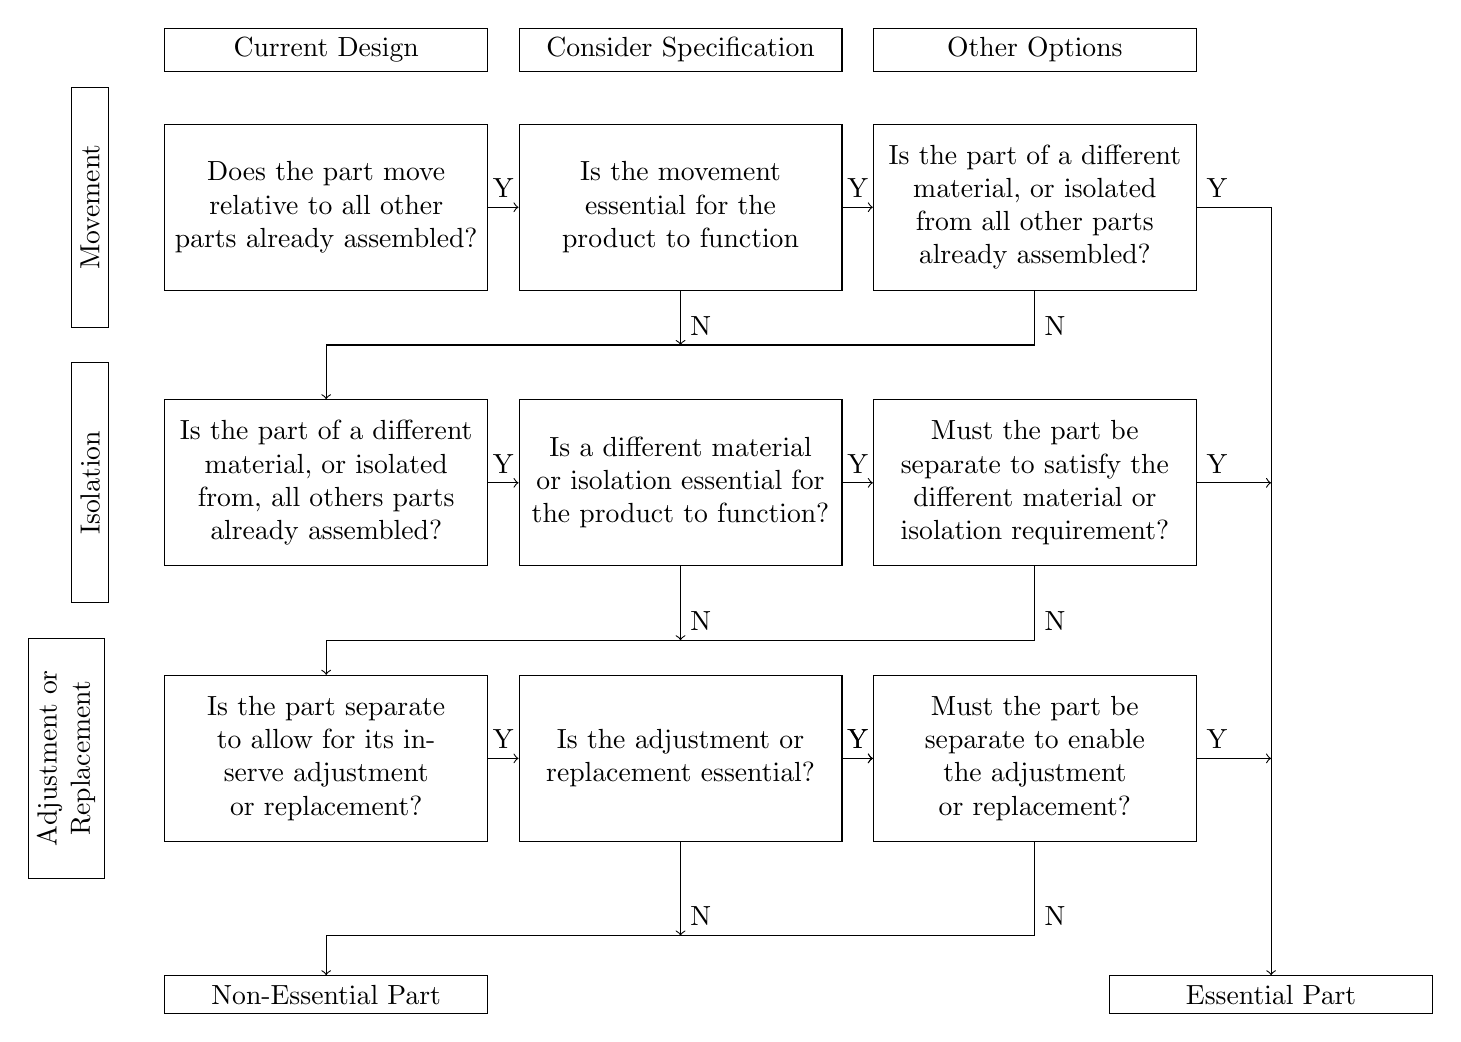
\begin{tikzpicture}%[scale=0.75, every node/.style={scale=0.75}]
      \node[align=center, draw, text width=110] at (0,0) {Current Design};

      \node[align=center, draw, text width=110] at (4.5,0) {Consider Specification};

      \node[align=center, draw, text width=110] at (9,0) {Other Options};

      \node[align=center, draw, text width=80, rotate=90] at (-3,-2) {Movement};

      \node[align=center, draw, text width=80, rotate=90] at (-3,-5.5) {Isolation};

      \node[align=center, draw, text width=80, rotate=90] at (-3.3,-9) {Adjustment or Replacement};

      \node[align=center, draw, text width=110, minimum height=60] (A) at (0,-2) {Does the part move relative to all other parts already assembled?};

      \node[align=center, draw, text width=110, minimum height=60] (B) at (4.5,-2) {Is the movement essential for the product to function};

      \node[align=center, draw, text width=110, minimum height=60] (C) at (9,-2) {Is the part of a different material, or isolated from all other parts already assembled?};

      \node[align=center, draw, text width=110, minimum height=60] (D) at (0,-5.5) {Is the part of a different material, or isolated from, all others parts already assembled?};

      \node[align=center, draw, text width=110, minimum height=60] (E) at (4.5,-5.5) {Is a different material or isolation essential for the product to function?};

      \node[align=center, draw, text width=110, minimum height=60] (F) at (9,-5.5) {Must the part be separate to satisfy the different material or isolation requirement?};

      \node[align=center, draw, text width=110, minimum height=60] (G) at (0,-9) {Is the part separate to allow for its in-serve adjustment or replacement?};

      \node[align=center, draw, text width=110, minimum height=60] (H) at (4.5,-9) {Is the adjustment or replacement essential?};

      \node[align=center, draw, text width=110, minimum height=60] (I) at (9,-9) {Must the part be separate to enable the adjustment or replacement?};

      \node[align=center, draw, text width=110] (J) at (0,-12) {Non-Essential Part};

      \node[align=center, draw, text width=110] (K) at (12,-12) {Essential Part};

      \draw[->] (A) -- (B) node[pos=0.5, anchor=south] {Y};
      \draw[->] (B) -- (C) node[pos=0.5, anchor=south] {Y};

      \draw[->] (D) -- (E) node[pos=0.5, anchor=south] {Y};
      \draw[->] (E) -- (F) node[pos=0.5, anchor=south] {Y};

      \draw[->] (G) -- (H) node[pos=0.5, anchor=south] {Y};
      \draw[->] (H) -- (I) node[pos=0.5, anchor=south] {Y};

      \draw[->] (H) -- (I) node[pos=0.5, anchor=south] {Y};

      \draw[->] (C) -- (9,-3.75) -| (D) node[pos=0, anchor=south west] {N};
      \draw[->] (B) -- (4.5,-3.75) node[pos=1, anchor=south west] {N};

      \draw[->] (F) -- (9,-7.5) -| (G) node[pos=0, anchor=south west] {N};
      \draw[->] (E) -- (4.5,-7.5) node[pos=1, anchor=south west] {N};

      \draw[->] (I) -- (9,-11.25) -| (J) node[pos=0, anchor=south west] {N};
      \draw[->] (H) -- (4.5,-11.25) node[pos=1, anchor=south west] {N};

      \draw[->] (C) -| (K) node[pos=0, anchor=south west] {Y};
      \draw[->] (F) -- (12,-5.5) node[pos=0, anchor=south west] {Y};
      \draw[->] (I) -- (12,-9) node[pos=0, anchor=south west] {Y};

    \end{tikzpicture}
    }
    \vspace{1em}
    \caption{Functional Analysis Chart}\label{fig-functional}
\end{figure*}

Alongside this, we need to assess whether there are any components that can be further standardised within the products. The level of standardisation is not critical at the moment and could be at the assembly, full assembly, assembly plant, corporation or industry levels. Then there is the question as to whether the part should be standardised. A `Yes' should only be placed next to part if both these criteria are met.

Having\marginnote{Part Count Efficiency $(\eta_{\text{part count}})$} calculated these values, we can begin to assess the performance of our current design. One metric that we use to assess a design is on it's part count efficiency. This is defined as the ratio between the theoretical number of parts required for the product to perform its function and actual number of parts within the design (\cref{equ-part-eff}).

\begin{equation}
  \eta_{\text{part count}} = \frac{\sum{N_\text{essential}}}{\sum{N_p}}
  \label{equ-part-eff}
\end{equation}


It is common that the designs following a DfA will have $\eta_{\text{part cout}}>0.6$ and this is the value that we will use as our objective.

In\marginnote{DfA Complexity Factor} addition to part count efficiency, we have the \ac{DfA} complexity factor, which is based on the number of parts and interactions within the design. It is calculated as the square root of the number of parts multiplied by the number of interactions.

\begin{equation}
  \text{Complexity Factor} = \sqrt{\sum{N_p}\times\sum{N_i}}
\end{equation} 


The objective of \ac{DfA} is to reduce this value, which can be achieved by reducing both the number of parts and interactions within the product. \cref{tbl-parts} shows an example output of Step 1.

\begin{table}[h!]
  \centering
  %\small
  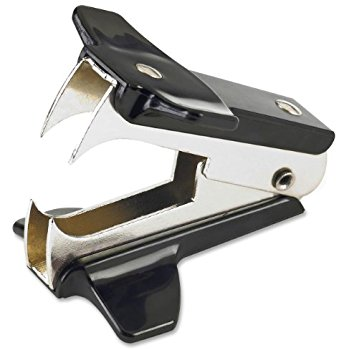
\includegraphics[width=0.3\textwidth]{figs/staple-remover.jpg} \\
  \footnotesize
  \begin{tabular}{l l r r c c}
    \toprule
      Part No. & Part Name & $N_p$ & $N_i$ & Essential &Standardised? \\
    \midrule
      1. & Lower Arm Sub-Assembly \\
    \midrule
      1.1 & Lower Arm & 1 & 6 & Y & N \\
      1.2 & Lower Arm Cover & 1 & 3 & N & Y \\
      1.3 & Rivet & 2 & 4 & N & N \\
    \midrule
      2. & Upper Arm Sub-Assembly & & \\
    \midrule
      2.1 & Upper Arm & 1 & 6 & N & N \\
      2.2 & Upper Arm Cover & 1 & 3 & N & Y \\
      2.3 & Rivet & 2 & 4 & N & N \\
    \midrule
      3. & Spring & 1 & 3 & N & N \\
    \midrule
      4. & Pivot & 1 & 3 & N & N \\
    \midrule
      Totals & & 10 & 32 & 1 & 2 \\
    \bottomrule
  \end{tabular}
  \caption{Staple remover functional analysis}\label{tbl-parts}
\end{table}


With\marginnote{Step Two} the functional analysis of the product complete, the next step is to calculate the assembly time for the product. This is not too much of a problem when you have an existing design that you're already manufacturing but can be challenging to estimate when you're early in the conceptual design phases.

To help us with determining the assembly time of components, researchers have performed studies into the time taken to perform common assembly tasks such as screwing components together, inserting bolts and handling time for small components. Figure~\ref{fig-screw} provides one such example.

\begin{figure}
    \centering
    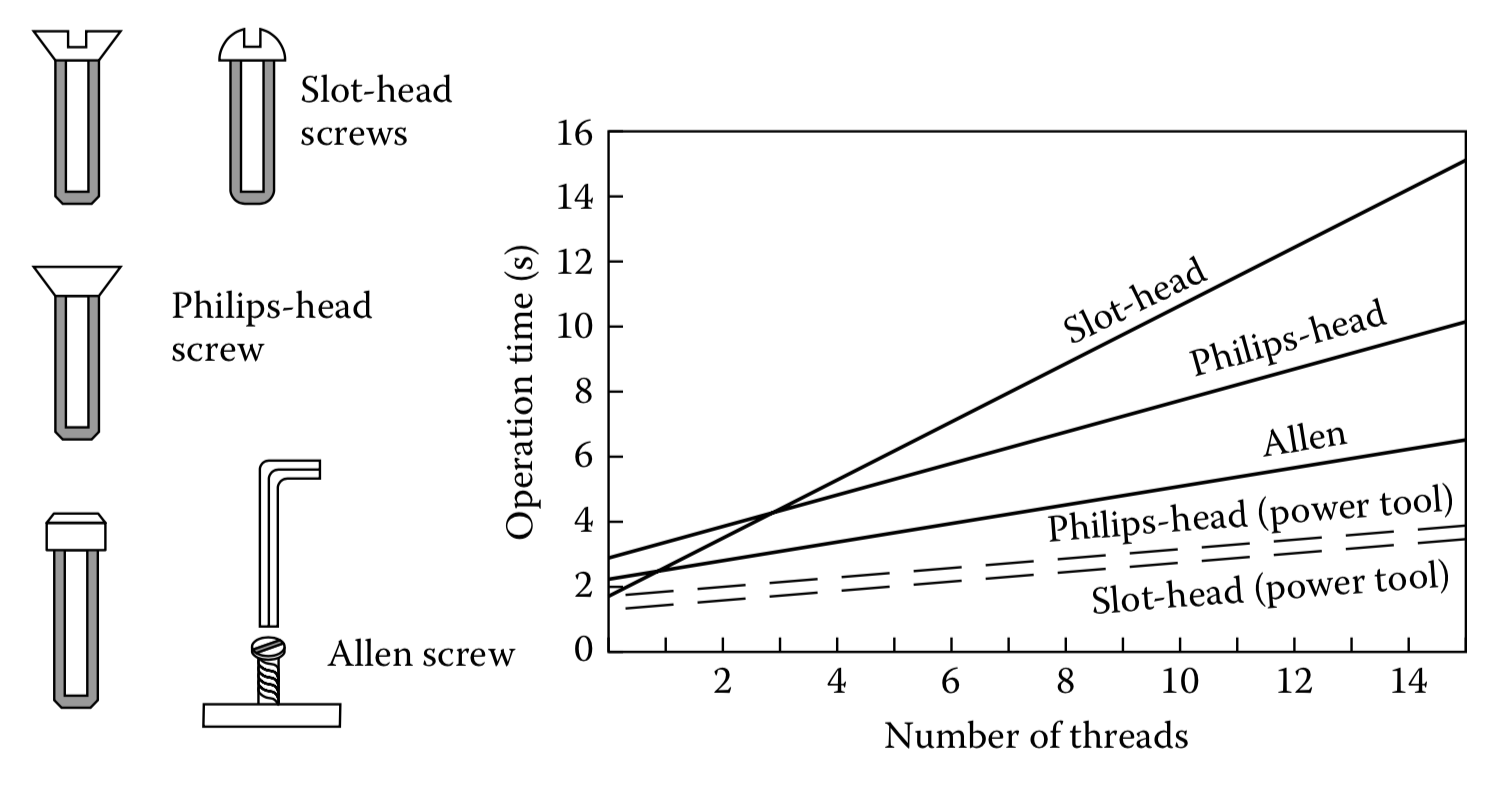
\includegraphics[width=\textwidth]{figs/screwing.png}
    \caption[Effect of number of threads on time to pick up the tool, engage the screw, tighten the screw, and replace the tool]{Effect of number of threads on time to pick up the tool, engage the screw, tighten the screw, and replace the tool~\citep{boothroyd2011}.}\label{fig-screw}
\end{figure}


From these charts, we can build an estimate for the assembly time for the current design. This forms the baseline that we can use to compare future iterations against.

\marginnote{Assembly Index} The assembly time can also be used to calculate the assembly index and is an indicator of the efficiency of the assembly process by comparing it to a theoretical minimum assembly time. This is obtained by multiplying the theoretical minimum part count of four by a minimum time of assembly for each part of 3s. 

\begin{equation}
  \text{Assembly index} = \frac{3\sum{N_i}}{\text{Assembly time}}
\end{equation}


With\marginnote{Step Three} our baseline set, we can begin to analyse and generate ideas of how we can improve the design for assembly. Step 3 is where we apply the \ac{DfA} guidelines to the current design and see if improvements can be made to ease its assembly.

It\marginnote{Component Elimination} is a rule of thumb that if a third of the components in a product are fasteners then one should look at the method of assembly. \cref{fig-bracket} shows an example of a roll-bar redesign where the number of parts has been reduced from 25 to 14.

\begin{figure*}[t!]
  \centering
  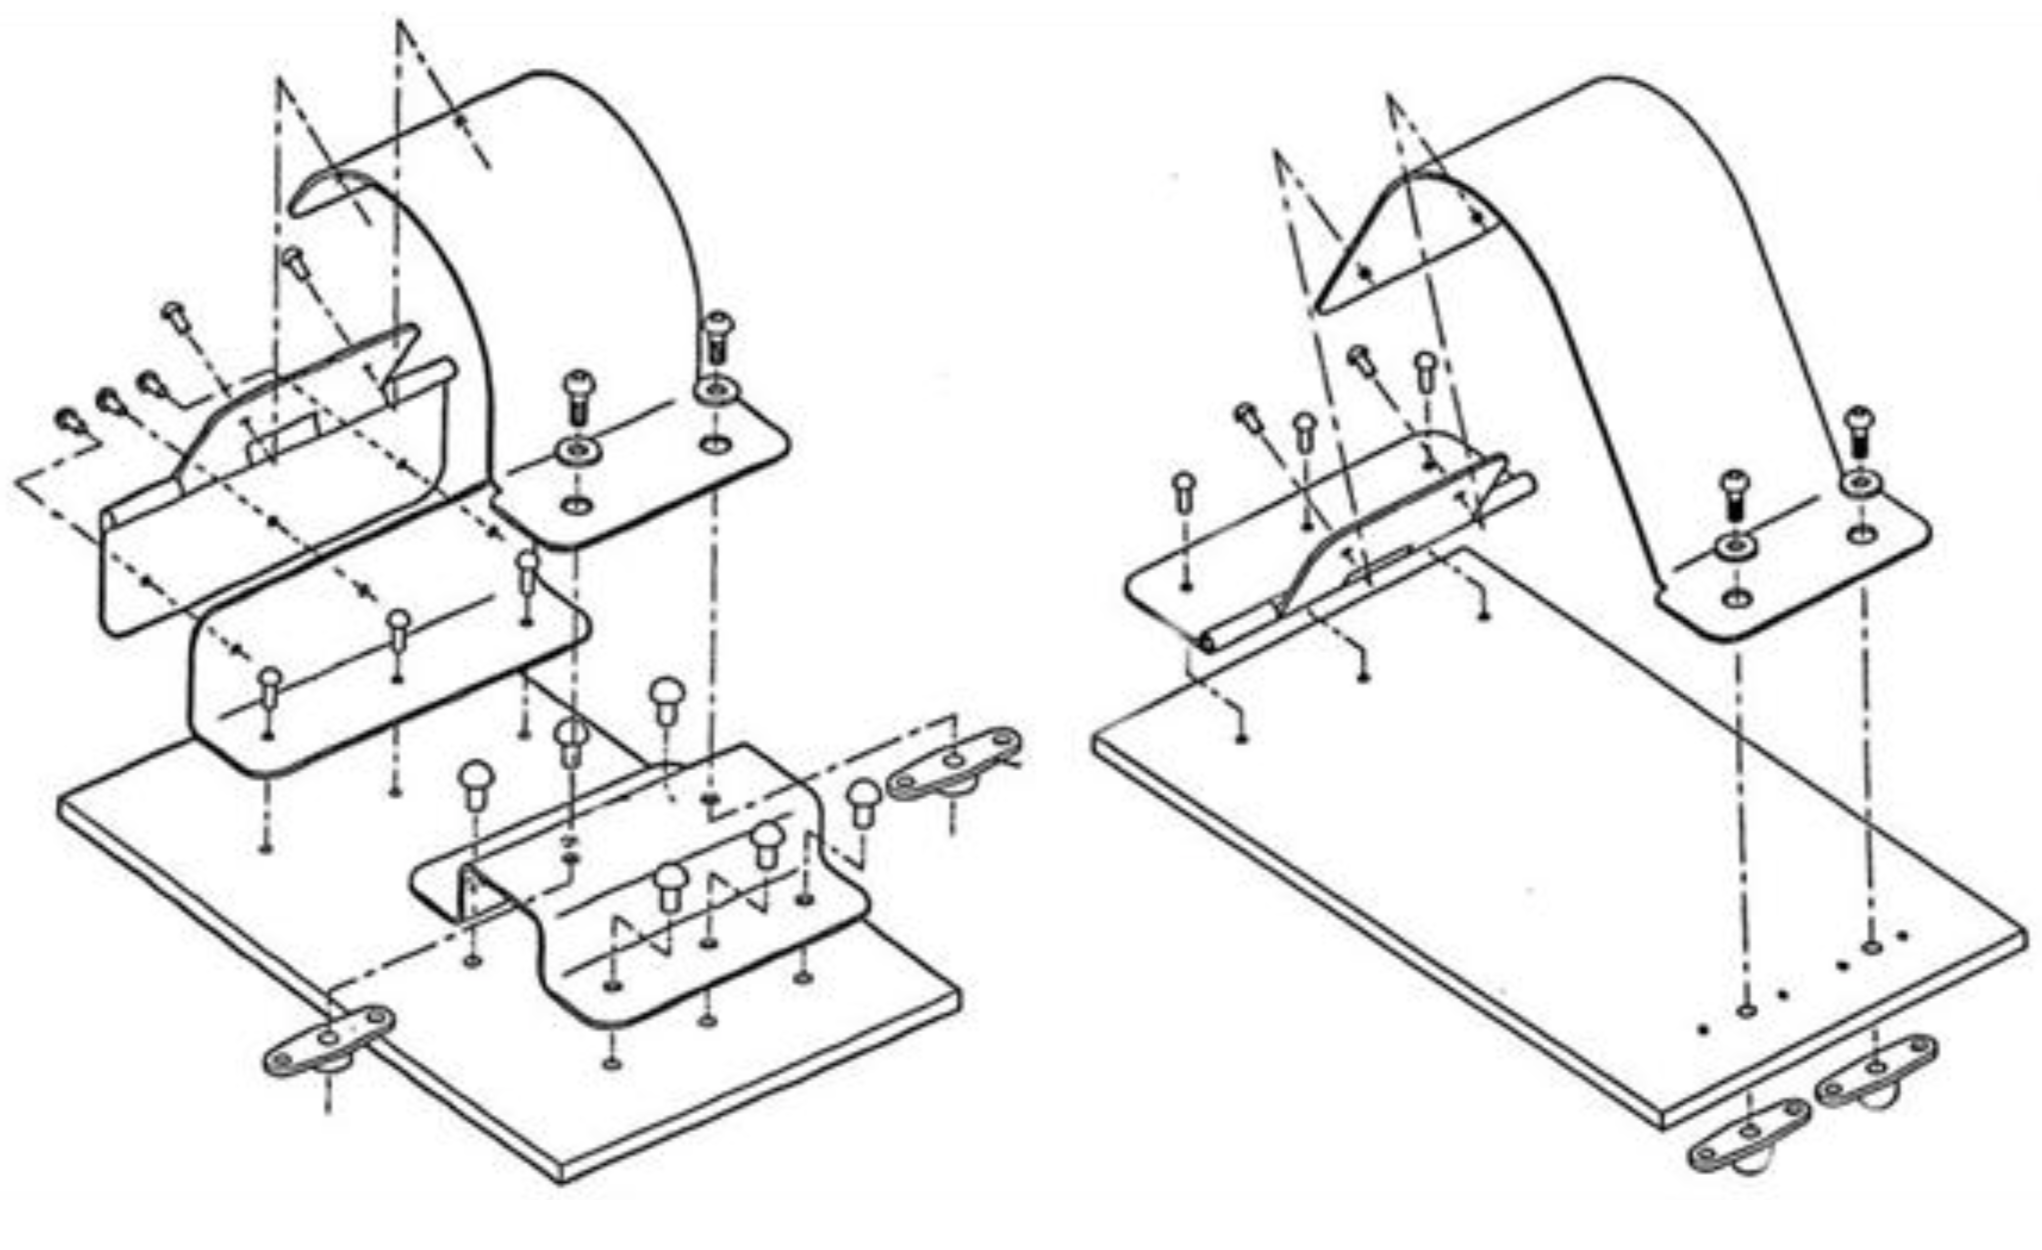
\includegraphics[width=0.8\textwidth]{figs/simplification.png}
  \caption{Simplification of a sheet metal bracket}\label{fig-bracket}
\end{figure*}


Remember, eliminated parts never need to be:

\begin{multicols}{3}
  \begin{itemize}
    \item Designed
    \item Detailed
    \item Prototyped
    \item Produced
    \item Scrapped
    \item Tested
    \item Re-engineered
    \item Purchased
    \item Progressed
    \item Received
    \item Inspected
    \item Rejected
    \item Stocked
    \item Outdated
    \item Written-off
    \item Unreliable
    \item Recycled
    \item Late
  \end{itemize}
\end{multicols}

However\marginnote{Standard Sizes}, there are times when fasteners are required and the number cannot be reduced further. In these cases, it is worth checking whether the types of fastener (e.g.\ bolt size) can be reduced. It is much easier for a company to stock one type of bolt than it is a hundred and simplifies the assembly time as there is less chance the wrong bolt is selected to mate two parts.

Fasteners\marginnote{Fastener Cost} also have an inherent cost in terms of the time it takes to assemble a component with them. Some of the lowest cost fasteners are snap fits requiring very little time and effort use. Whilst bolting requires additional equipment and many turns until the two parts are assembled. In addition, they may be the need to torque the bolt to a specific level, which further increases the assembly time.

In\marginnote{Part Handling} general, for ease of part handling, a design engineer should attempt to:

\begin{enumerate}
  \item Design parts that have an end-to-end symmetry and rotational symmetry about the axis of insertion. If this cannot be achieved, try to design parts having the maximum possible symmetry (\cref{fig-handling}a).
  \item Design parts that, in those instances where the part cannot be made symmetric, are obviously asymmetric (\cref{fig-handling}b).
  \item Provide features that prevent jamming of parts that tend to nest or stack when stored in bulk (\cref{fig-handling}c).
  \item Avoid features that allow tangling of parts when stored in bulk (\cref{fig-handling}d).
  \item Avoid parts that stick together or are slippery, delicate, very small or very large, or that are hazardous to the handler (i.e.\ parts that are sharp, splinter easily, etc.)
\end{enumerate}

\begin{figure}[t!]
  \centering
  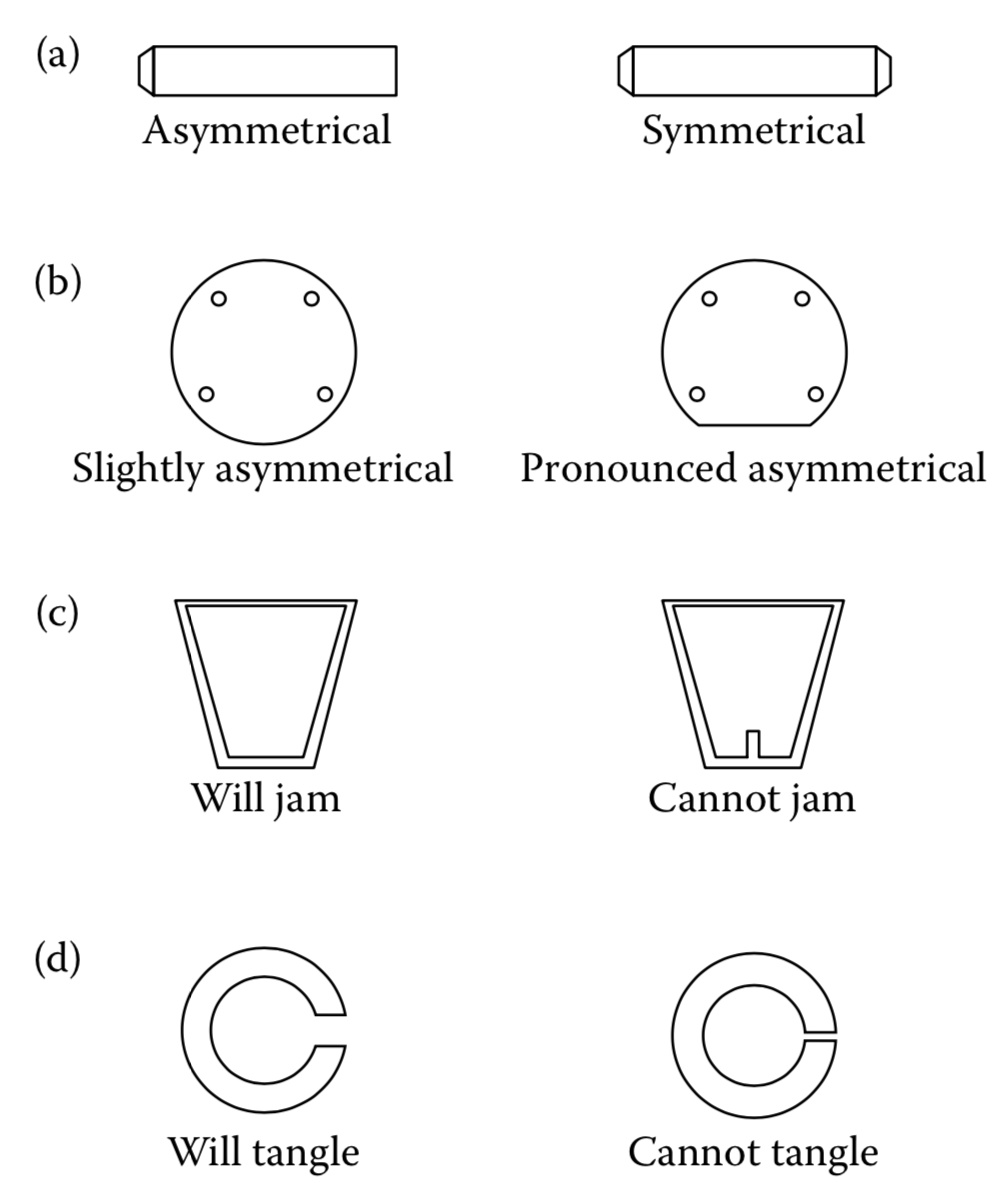
\includegraphics[width=0.6\textwidth]{figs/handling.png}
  \caption[Geometric features that effect part handling]{Geometric features that effect part handling~\citep{boothroyd2011}.}\label{fig-handling}
\end{figure}



\marginnote{Insertion and Fastening} For ease of insertion, an engineer should attempt to:

\begin{enumerate}
  \item Design so that there is little or no resistance to insertion and provide chamfers to guide the insertion of two mating parts. Generous clearance should be provided, but care must be taken to avoid clearances that result in a tendency for parts to jam or hang-up during insertion.
  \item Standardize by using common parts, processes, and methods across all models and even across product lines to permit the use of higher volume processes that normally result in lower product cost.
  \item Use pyramid assembly to provide progressive assembly about one axis of reference. In general, it is best to assemble from above.
  \item Avoid, where possible, the necessity for holding parts down to maintain their orientation during manipulation of the sub-assembly or during the placement of another part. If holding down is required, then try to design so that the part is secured as soon as possible after it has been inserted.
  \item Design so that a part is located before it is released. A potential source of problems arises from a part being placed where, due to design constraints, it must be released before it is positively located in the assembly. Under these circumstances, reliance is placed on the trajectory of the part being sufficiently repeatable to locate it consistently.
  \item When common mechanical fasteners are used, the following sequence indicates the relative cost of different fastening processes, listed in the order of increasing manual assembly cost.
  \begin{enumerate}
    \item Snap fits
    \item Plastic bending
    \item Riveting
    \item Screw fastening
  \end{enumerate}
  \item Avoid the need to reposition the partially completed assembly in the jig.
\end{enumerate}

By\marginnote{Step Four} evaluating your designs with respect to these guidelines, new design should emerge that will ease the assembly of the product. To evaluate the relative success of the DfA activity, we now perform Steps 1 \& 2 again for the new design and compare it with the old version.

To demonstrate the potential improvements that can be gained by performing this activity, \cref{fig-motor} illustrates the design changes that were made to a motor drive assembly. And, \cref{tbl-comparison} shows the comparison of the original motor design against the re-design motor assembly. The results show a:

\begin{itemize}
  \item 68\% reduction in the number of parts required;
  \item 70\% reduction in assembly time; and,
  \item 71\% reduction in labour costs.
\end{itemize}


\begin{figure*}[ht!]
    \centering
    \begin{tabular}{c c}
      \subfloat[Original design]{
        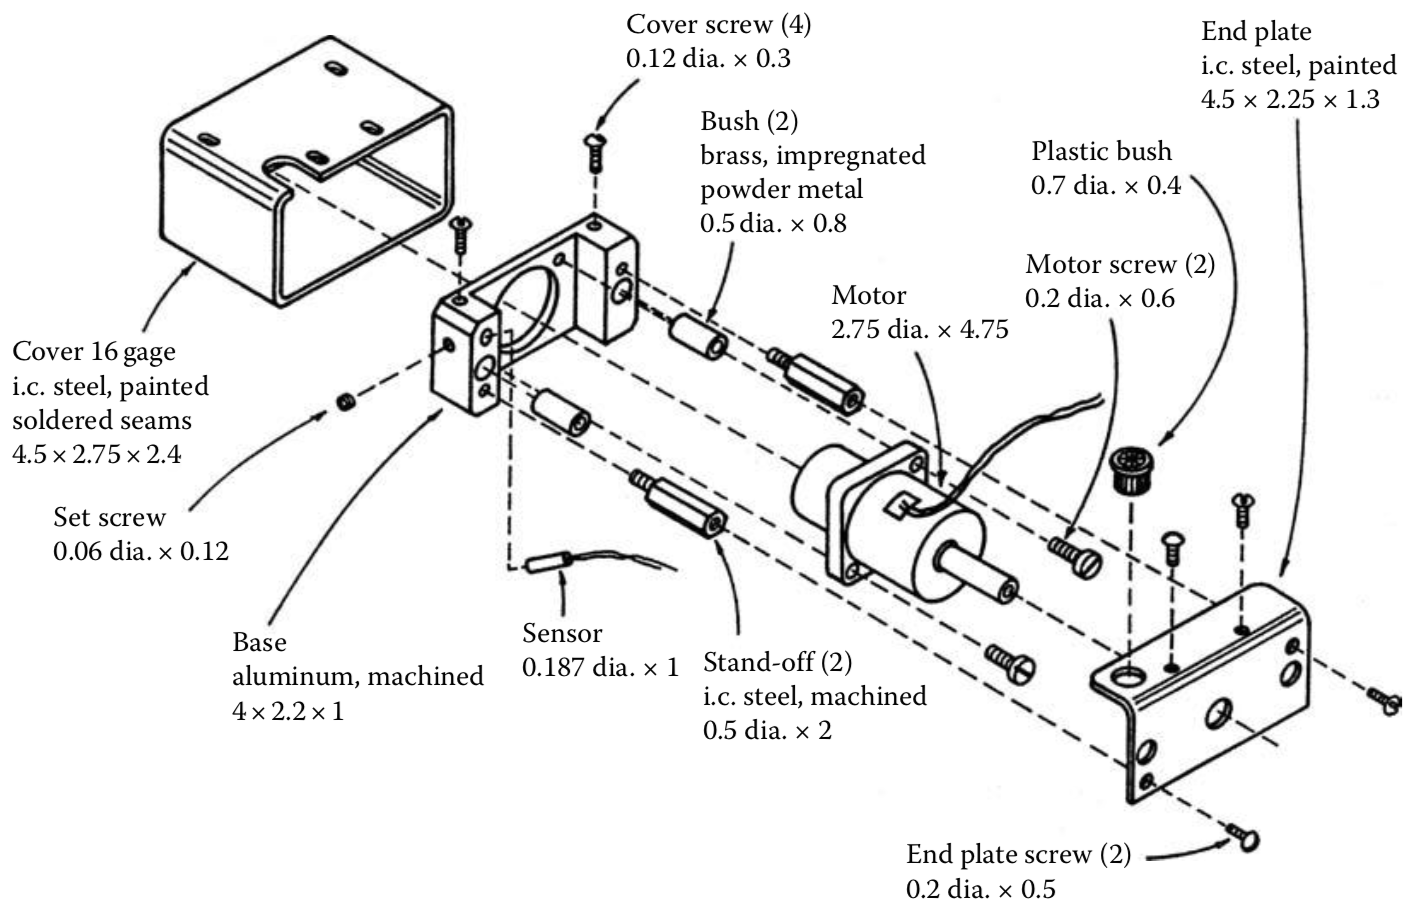
\includegraphics[width=0.43\textwidth]{figs/motor-1.png}
      } & 
      \subfloat[Re-design]{
        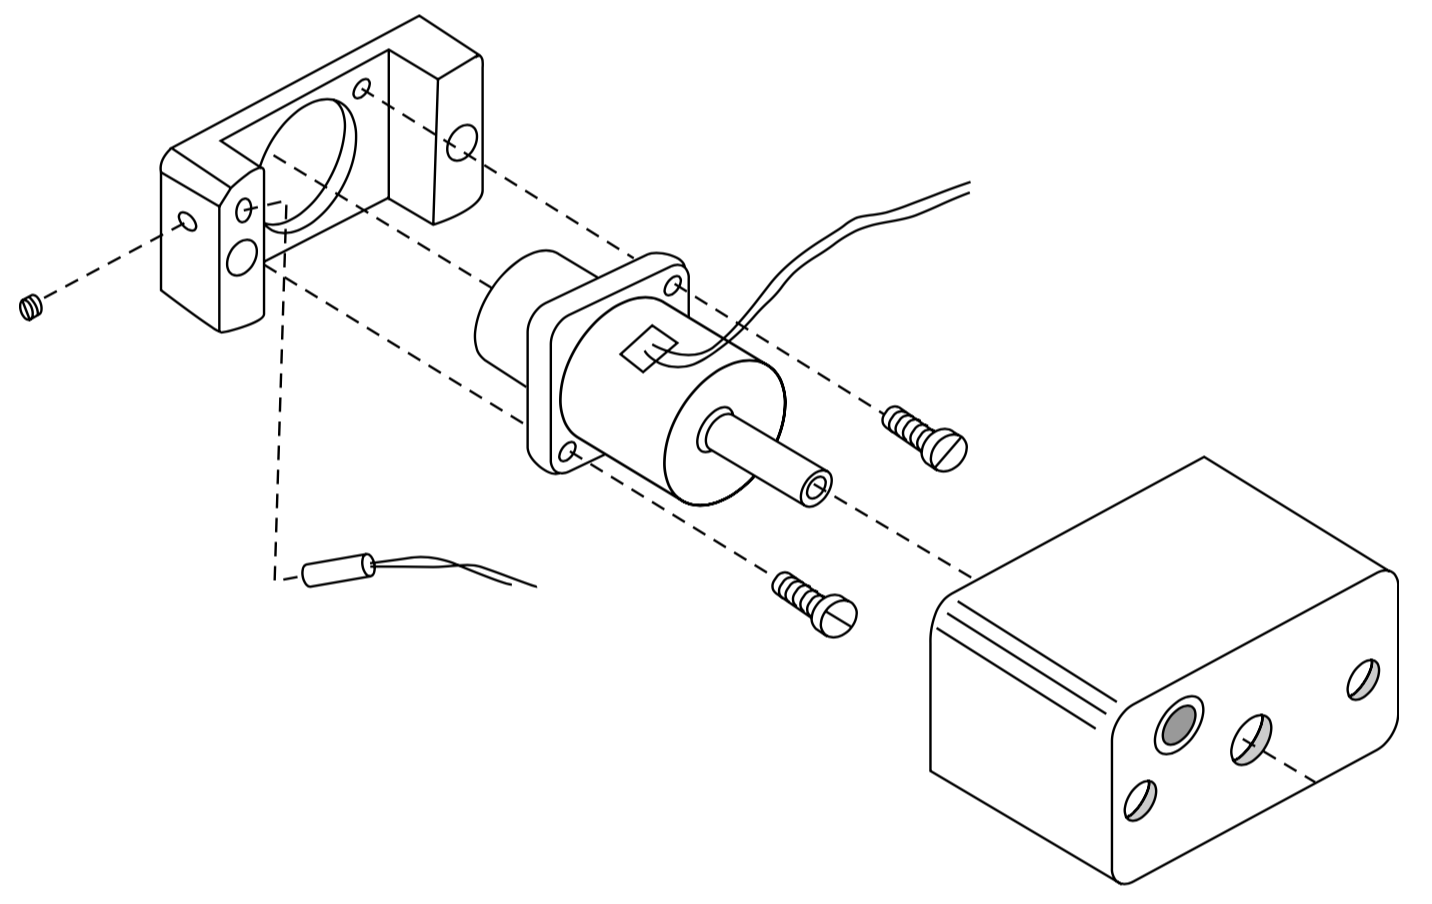
\includegraphics[width=0.43\textwidth]{figs/motor-2.png}
      }
    \end{tabular}
    \vspace{1em}
  \caption{Motor drive assembly DfA re-design}\label{fig-motor}
\end{figure*}

\begin{table*}[ht!]
    \centering
    \resizebox{\textwidth}{!}{
    \scriptsize
    \begin{tabular}{l | r r | r r | r r | r r}
      \toprule
        Part & \multicolumn{2}{c|}{$N_p$} & \multicolumn{2}{c}{$N_i$} & \multicolumn{2}{c}{Assembly Time (s)} & \multicolumn{2}{c}{Assembly Cost (\textdollar)*} \\
        & Original & Re-Design & Original & Re-Design & Original & Re-Design & Original & Re-Design \\
      \midrule
        Base & 1 & 1 & 1 & 1 & 3.5 & 3.5 & 2.9 & 2.9 \\
        Bushing & 2 & -- & 0 & -- & 12.3 & -- & 10.2 & -- \\
        Motor sub-assembly & 1 & 1 & 1 & 1 & 9.5 & 4.5 & 7.9 & 3.8 \\
        Motor screw & 2 & 2 & 0 & 0 & 21.0 & 12.0 & 17.5 & 10.0 \\
        Sensor sub-assembly & 1 & 1 & 1 & 1 & 8.5 & 8.5 & 7.1 & 7.1 \\
        Set screw & 1 & 1 & 0 & 0 & 10.6 & 8.5 & 8.8 & 7.1 \\
        Standoff & 2 & -- & 0 & -- & 16.0 & -- & 13.3 & -- \\
        End plate & 1 & -- & 1 & -- & 8.4 & -- & 7.0 & -- \\
        End plate screw & 2 & -- & 0 & -- & 16.6 & -- & 13.8 & -- \\
        Plastic bushing & 1 & -- & 0 & -- & 3.5 & -- & 2.9 & -- \\
        Thread leads & -- & -- & -- & -- & 5.0 & 5.0 & 4.2 & 4.2 \\
        Reorient & -- & -- & -- & -- & 4.5 & -- & 3.8 & -- \\
        Cover & 1 & 1 & 0 & 1 & 9.4 & 4.0 & 7.9 & 3.3 \\
        Cover screw & 4 & -- & 0 & -- & 31.2 & -- & 26.0 & -- \\
        \midrule
        Totals & 19 & 6 & 4 & 4 & 160.0 & 46.0 & 133.0 & 38.4 \\
      \bottomrule
      \multicolumn{5}{l}{*labour cost at \textdollar30ph} \\
    \end{tabular}
    }
    \vspace{1em}
    \caption{Motor DfA comparison}
    \label{tbl-comparison}
\end{table*}


\subsection{Design for Manufacture (Laser Cutting)}

Laser\marginnote{\normalfont Acknowledgements to Sculpteo's ``Laser Cutting: The Ultimate Guide''} cutting works by directing the output of a high-power laser through optics. They direct the laser beam generated on a small zone of the material. The material then either melts, burns, vaporizes away, or is blown away by a jet of gas, leaving an edge with a good quality surface finish. Typical prototyping laser cutters can cut up to \SI{20}{\milli\metre} thick material.

Laser cutting machines function from digital orders, based on the topographic information contained in a 2-D vector file. They cut or engrave the material plate in different locations, thus allowing an item's surface to be delineated and decorated.

\subsubsection{Origins of Laser Cutting}

One\marginnote{1965} of the earliest known applications of laser technology in manufacturing was as a cutting device for electrical connections. This had been previously achieved through diamond dies and many thousands were used in the process. Diamond dies were both costly and time consuming to make. Cutting with laser technology overcame this barrier but there were still concerns over its safety.

In 1967\marginnote{1967}, Peter Houldcroft of the The Welding Institute in Cambridge discovered that combining a focused laser beam with an oxygen assist gas could improve the precision and speed by the cutting process. This led to the development of the laser cutting nozzle we know today\cite{sullivan1967}.

Industrial\marginnote{1969} application of laser cutting technologies started to be realised with Boeing becoming one of the first to integrate the technology within its production lines. The focus was on the development of the technology to cut `hard' material such as titanium, hastelloy and ceramic. There results led to the patenting of multi-beam laser cutting.

Now\marginnote{1979} laser cutting had become synonymous of cutting in two dimensions and it wasn't until 1979 when Italian company Prima Industrie demonstrated that it was possible to use the technology in a three-dimensions by placing the process on a 5-axis rotation system.

Fast\marginnote{Today} forward to today and laser cutters have fully-established themselves as a viable manufacturing technology in both prototyping and production. The technology has also shrunk to the size that you can fit one on your desktop. It is used in a range of sectors including marketing, solar panel construction and aerospace. And now in the Design \& Make exercise!

\subsubsection{Laser Cutting Process}

\cref{fig-cutter} shows a schematic of the laser cutting process. The laser originates from a laser resonator, which sends out a beam of intense light that is reflected through a system of mirrors to the cutting head. Within the cutting head, the laser is focused through a lens and narrowed down to an extremely thin, concentrated beam.

\begin{figure}
  \centering
  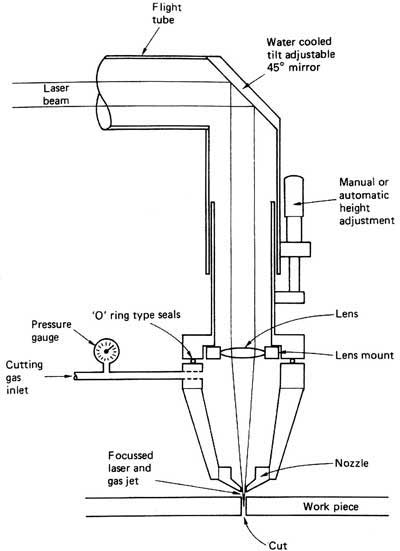
\includegraphics[width=0.6\textwidth]{figs/laser-cutter.jpg}
  \caption{Schematic of a laser cutter}\label{fig-cutter}
\end{figure}

Movement is often achieved though either a gantry system where a laser beam is placed perpendicularly to the materials and the beam is directed by three mirrors: one static and two mobile, or a galvanometer system.


\subsubsection{Guidelines}

You\marginnote{Use Material Wisely} will most likely use a full-size sheet for every run you require. So remember to think about how to optimise that use of material. If you know that you will be laser cutting a number of components, try and make them using the same thickness and type of material so that they can be all positioned on the same sheet. This will minimise set-up and change over times. Packing algorithms do exist that optimise positioning of components on two dimensional sheets. The first-fit decreasing height algorithm is one such example.

It\marginnote{Print It Out!} might sound obvious but it's always good to print out your potential laser cut designs so you can check for any issues that might come about through scaling or having selected the wrong units in your CAD software.

The\marginnote{Think about Material Thickness} thicker the material, the longer it will take to cut and cost. It's always good to consider the forces that will be flowing through the part. Smaller thicknesses will speed up prototyping.

Laser\marginnote{Check for Narrow Gaps} cutters typically remove \SI{0.2}{\milli\metre} of material along the line it is tracing (kerf). Therefore, avoid designing parts that have lines with gaps narrower than \SI{1}{\milli\metre} as these will be weak and have a greater chance of breaking.

The\marginnote{Remember the Kerf when Making Assembly Slots} kerf can also effect the fit between your parts. Make sure you take this into consideration when developing your CAD models. You may have a version that fits perfectly on CAD but you may have to create another version of the parts to compensate for the laser cutter.

There\marginnote{Engrave you Group Number and Part Id} will be a lot of parts being laser cut over the summer holidays and you'll have a number of parts that will look similar. Adding an engraving will help identify the parts when you come to build next year.


\subsection{Design for Manufacture (3D Printing)}

3D printing refers to processes in which material is joined or solidified under computer control to create a three-dimensional object. The term is often used interchangeably with Rapid Prototyping and Additive Manufacturing but we tend to use 3D Printing to describe low-cost additive manufacturing systems. And research at the University of Bath has been instrumental in creating low-cost 3D printing.

\begin{marginfigure}
  \centering
  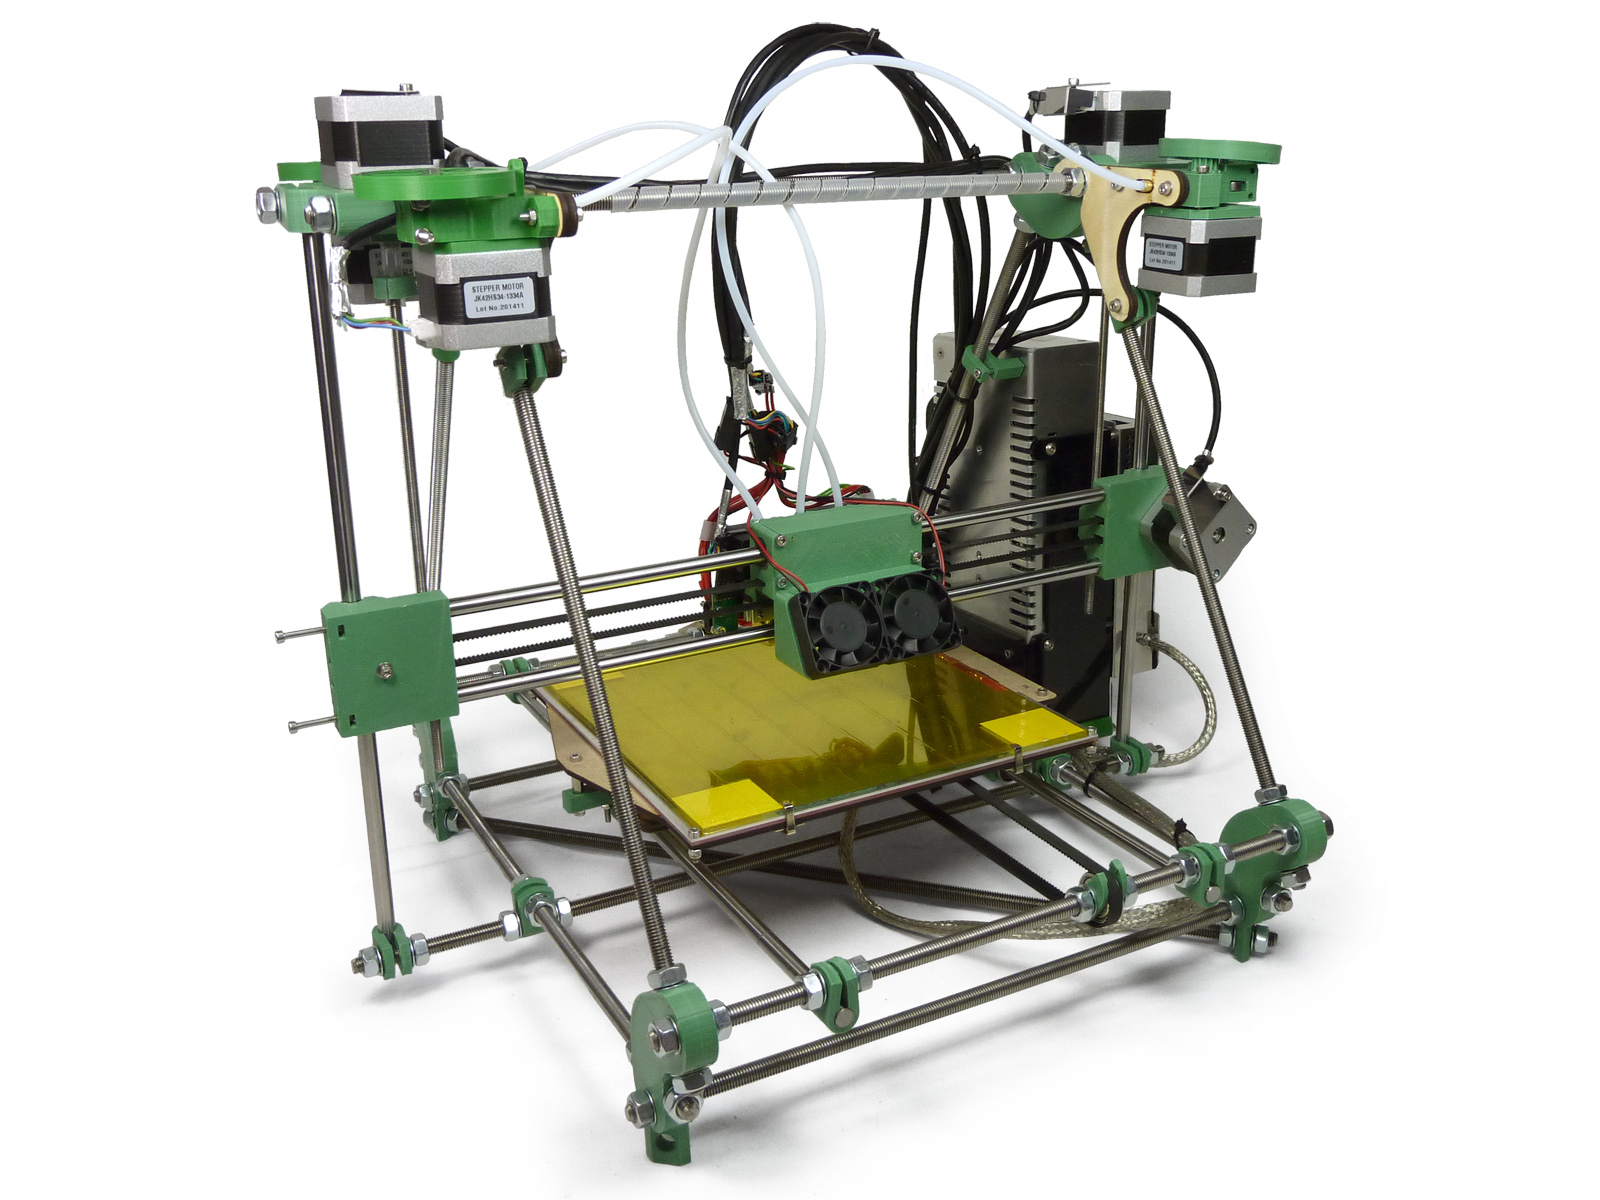
\includegraphics[width=\textwidth]{figs/mendel.jpg}
  \caption{Mendel RepRap 3D Printer}
  \label{fig-reprap}
\end{marginfigure}

The work by Dr Bowyer and his colleagues on the open-source RepRap project (\cref{fig-reprap}) has led to the technology that has been implemented in the majority of low-cost Fused Deposition Modelling (FDM) printers on the market today.~\cite{jones2011}


\subsubsection{Types}

There are a number of different types of 3D printing but the most commonly used techniques in rapid prototyping are \acf{FDM} and \acf{SLS}.

\ac{FDM}\marginnote{Fused Deposition Modelling (FDM)}, also known as \acf{FFF} is a 3D printing process that uses a continuous filament of a thermoplastic material. This is fed from a large coil, through a moving, heated extrusion head. The head is \acf{CNC} with the input often being GCode that is turned to machine code to operate the stepper motors on the machine. Extruder temperatures are in the region of \SI{200}{\degreeCelsius}, filament diameters are around \SI{2.85}{\milli\metre} and deposition rates are around \SI{20}{\milli\metre\per\second}.

\ac{SLS}\marginnote{Selective Laser Sintering (SLS)} is a technique that uses a laser to sinter powdered materials. Layers of powdered material is deposited on a bed and after each pass, the laser is directed towards the areas that have been defined in the 3D model as solid geometry. \acf{DMLS} and \acf{SLM} all follow a similar process. The technique was developed and patented by Dr. Deckard in the mid-1980s. The fine-grain structure and accuracy of the laser sintering process enables high-quality prototypes to be generated however, the structural strength of the component is highly-dependent on how well the layers fuse together and there remains is issues when high-tolerances are concerned.

The section now focuses on \ac{FDM} as this is the method that is available to you for your project.


\subsubsection{Terminology}

The\marginnote{Slicing} procedure of taking a \acf{CAD} model and producing the relevant code for the printer to print the model. Users often need to export their \ac{CAD} model as an \acf{STL} file and this is imported into the slicing tool. There are a range of slicing tools that are available and some of the most common are:

\begin{itemize}
  \item Cura
  \item MakerWare
  \item MatterControl
  \item Repetier
  \item Slic3r
\end{itemize}

Research at the University of Bath is leading the development of slicing tools that optimise the internal geometry of printed parts based on the predicted loads through the part (Figure~\ref{fig-3d-print-bath})~\cite[-3em]{pam2017}.

\begin{figure*}
    \center{}
    \begin{tabular}{c c}
      \subfloat[FEA]{
        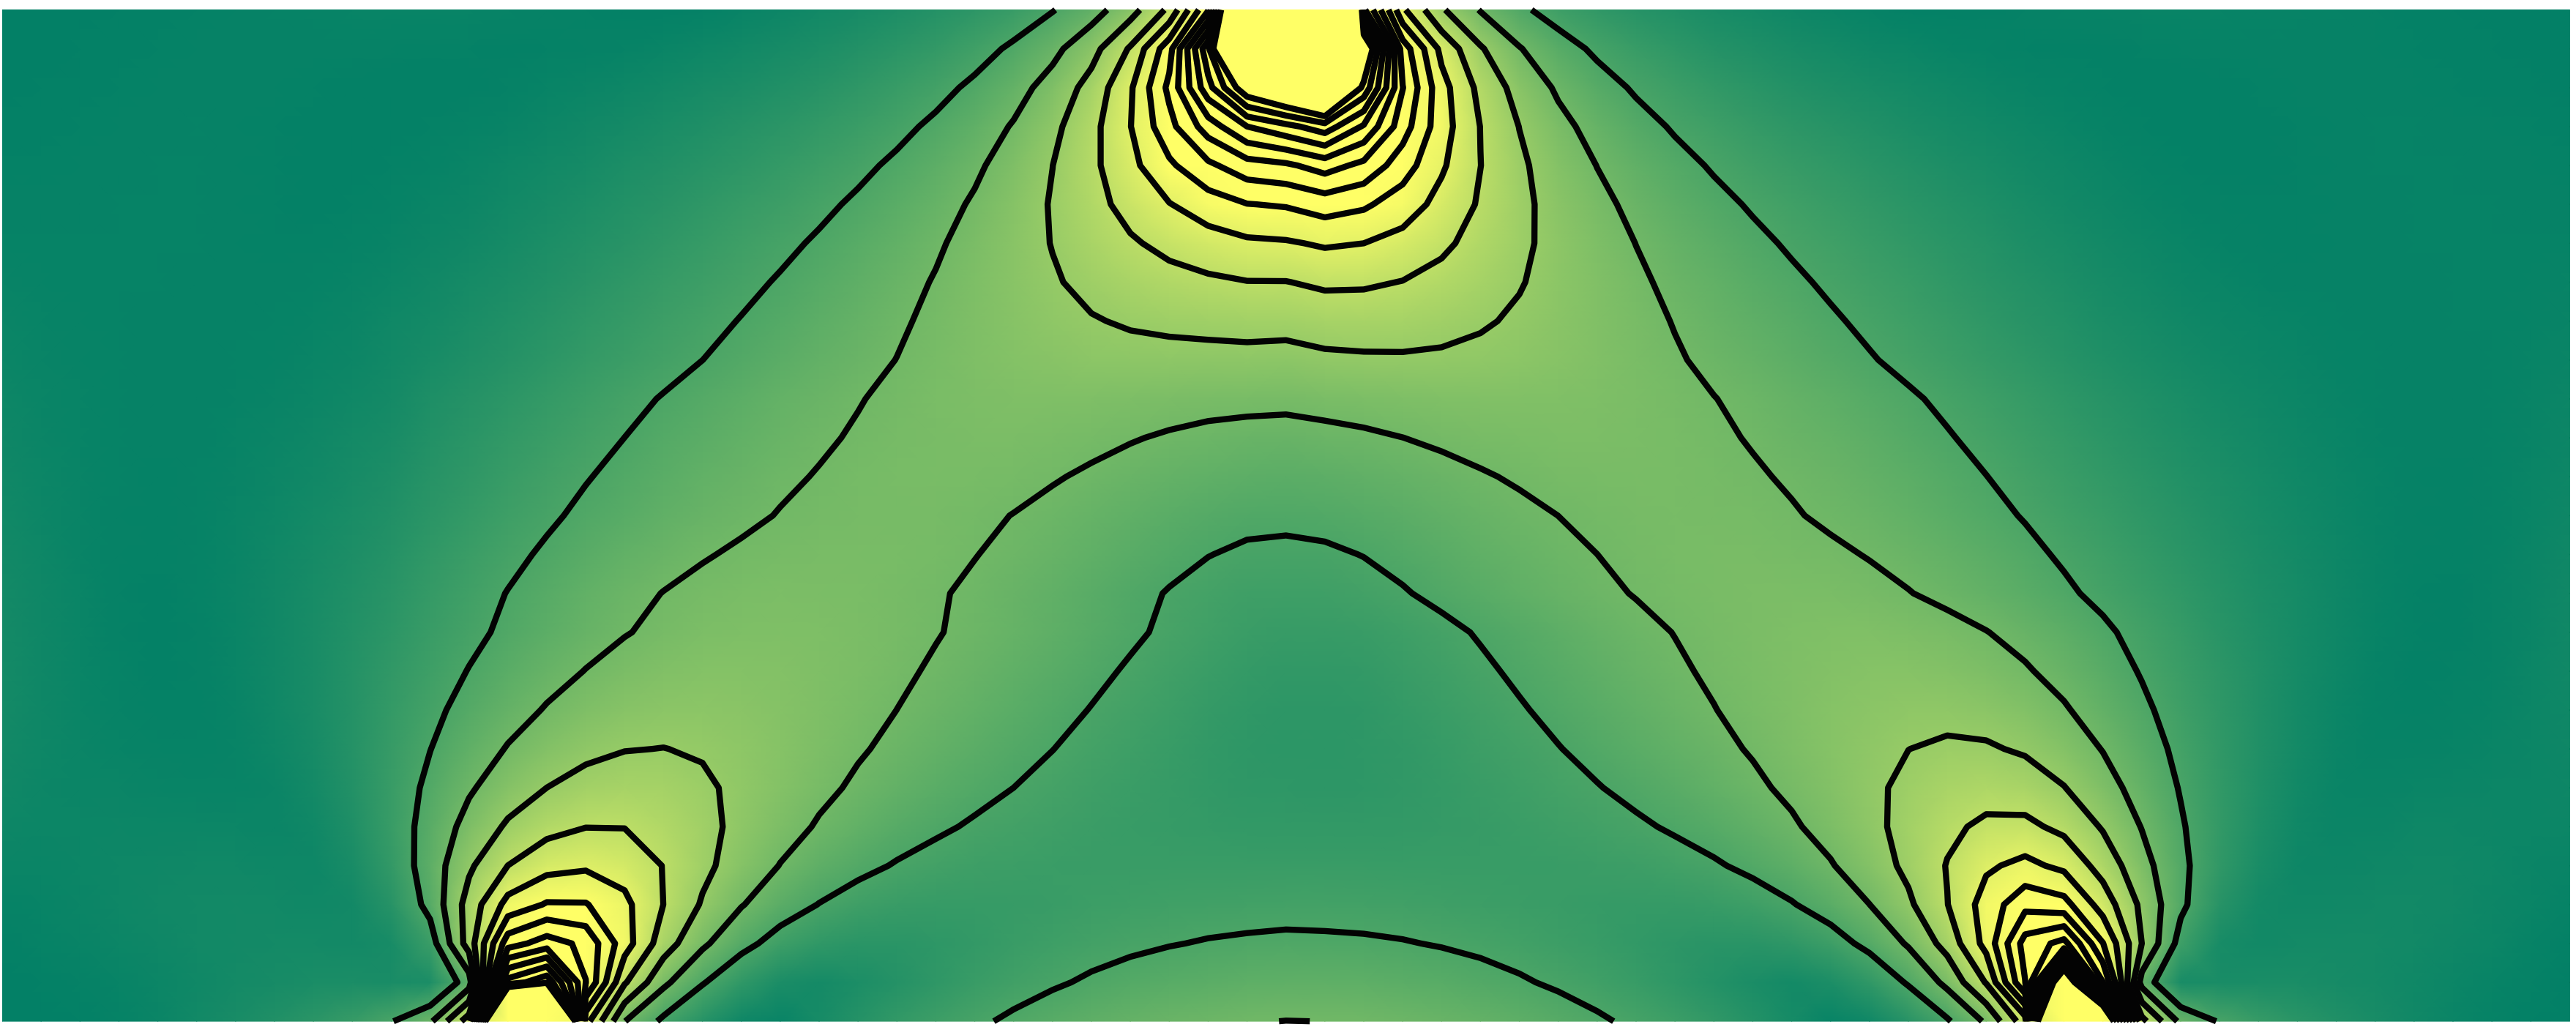
\includegraphics[width=0.45\textwidth]{figs/fea_three_point_beam.png}
      }
      &
      \subfloat[Infill Design]{
        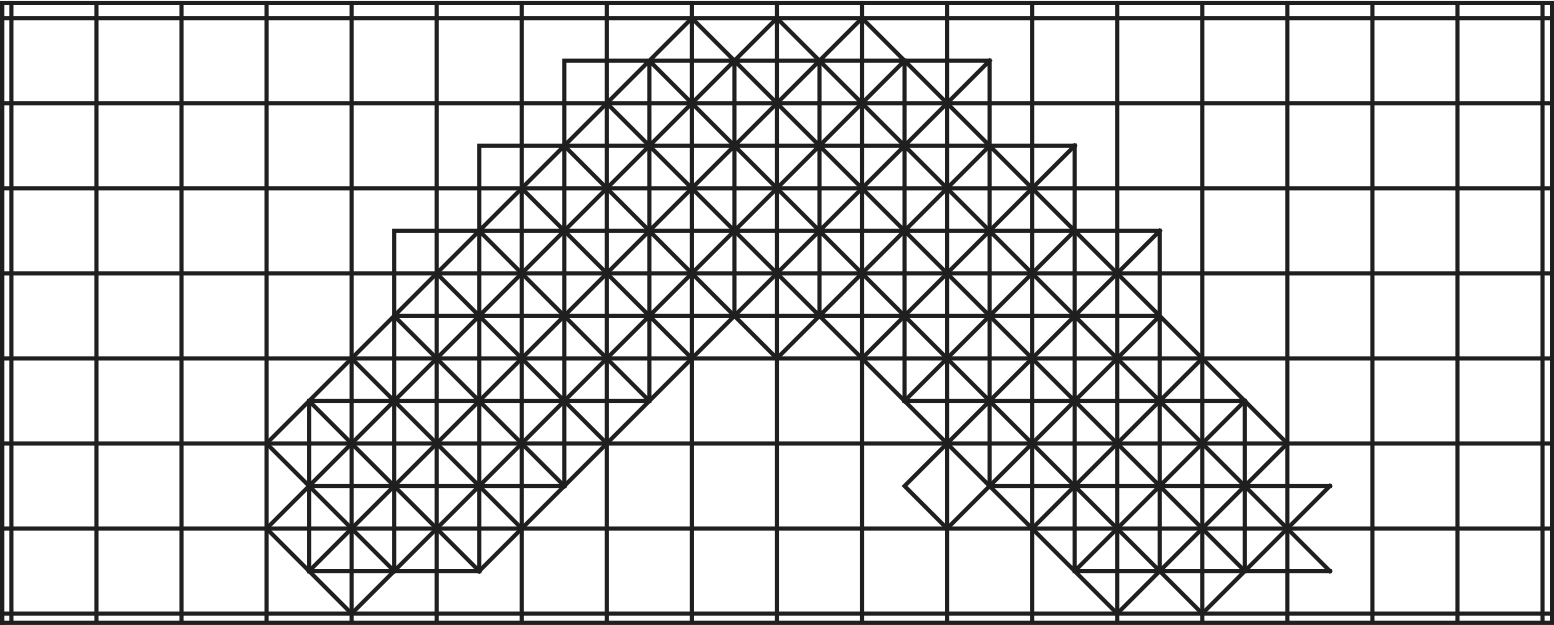
\includegraphics[width=0.45\textwidth]{figs/three_point_beam.png}
      }
    \end{tabular}
    \vspace{1em}
    \caption{Optimised Lattice Infill for a Three-Point Bend Test}
    \label{fig-3d-print-bath}
\end{figure*}



Slicing tools provide a range of options that aid the user in optimising the print time and material use in creating the prototype. The main options are the number of shells, infill design/density, rafts and supports.

Shells\marginnote[1em]{Shells} are the number of times the 3D printer will print the external geometry of the slice.

Infill\marginnote{Infill} is the design of the internal geometry for the 3D printed part (\cref{fig-infills}). Each infill can have its density adjusted with 100\% being a solid printed part and 0\% being a part within no internal infill. The typical value for infill density is 20\%, which provides a suitable compromise between part strength and print time.

\begin{figure*}[t!]
  \center{}
  \begin{tabular}{p{0.16\textwidth} p{0.16\textwidth} p{0.16\textwidth} p{0.16\textwidth} p{0.16\textwidth}}

  \subfloat[Linear]
  {
  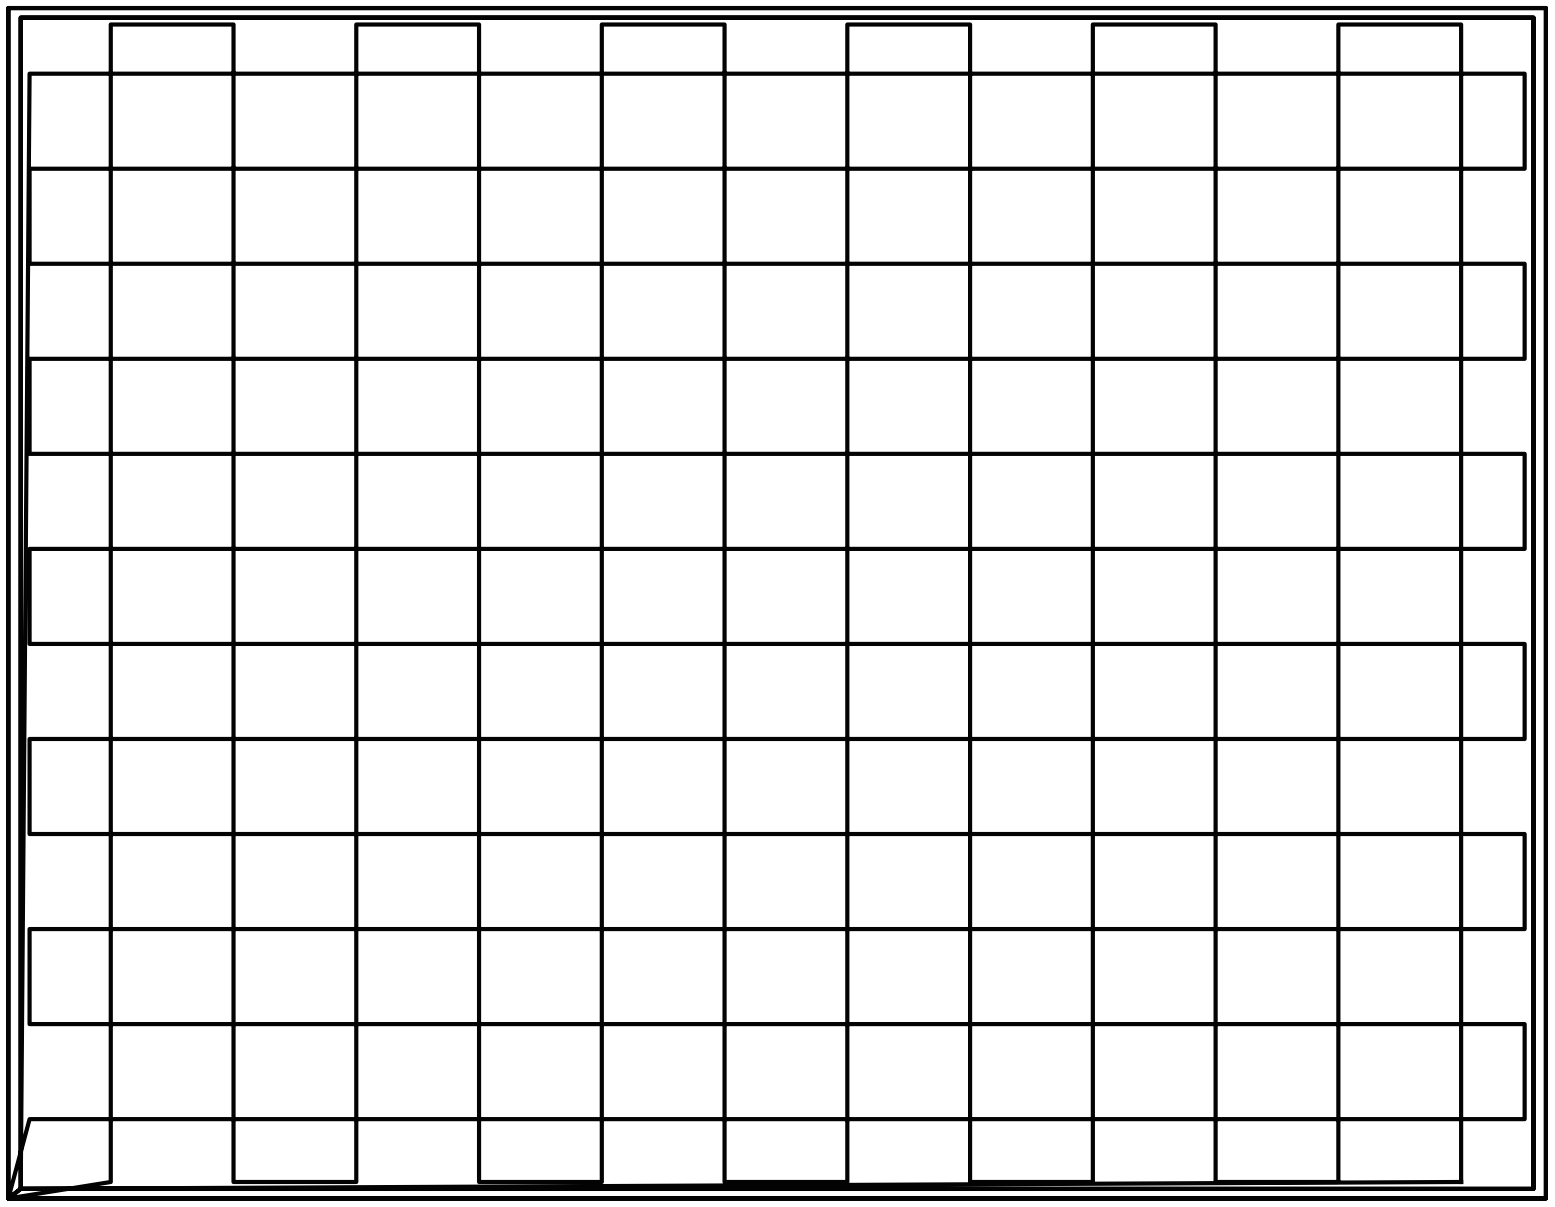
\includegraphics[width=0.18\textwidth]{figs/makerbot_infill_strategy_square_linear.png}
  \label{}
  }
  &
  \subfloat[Hexagonal]
  {
  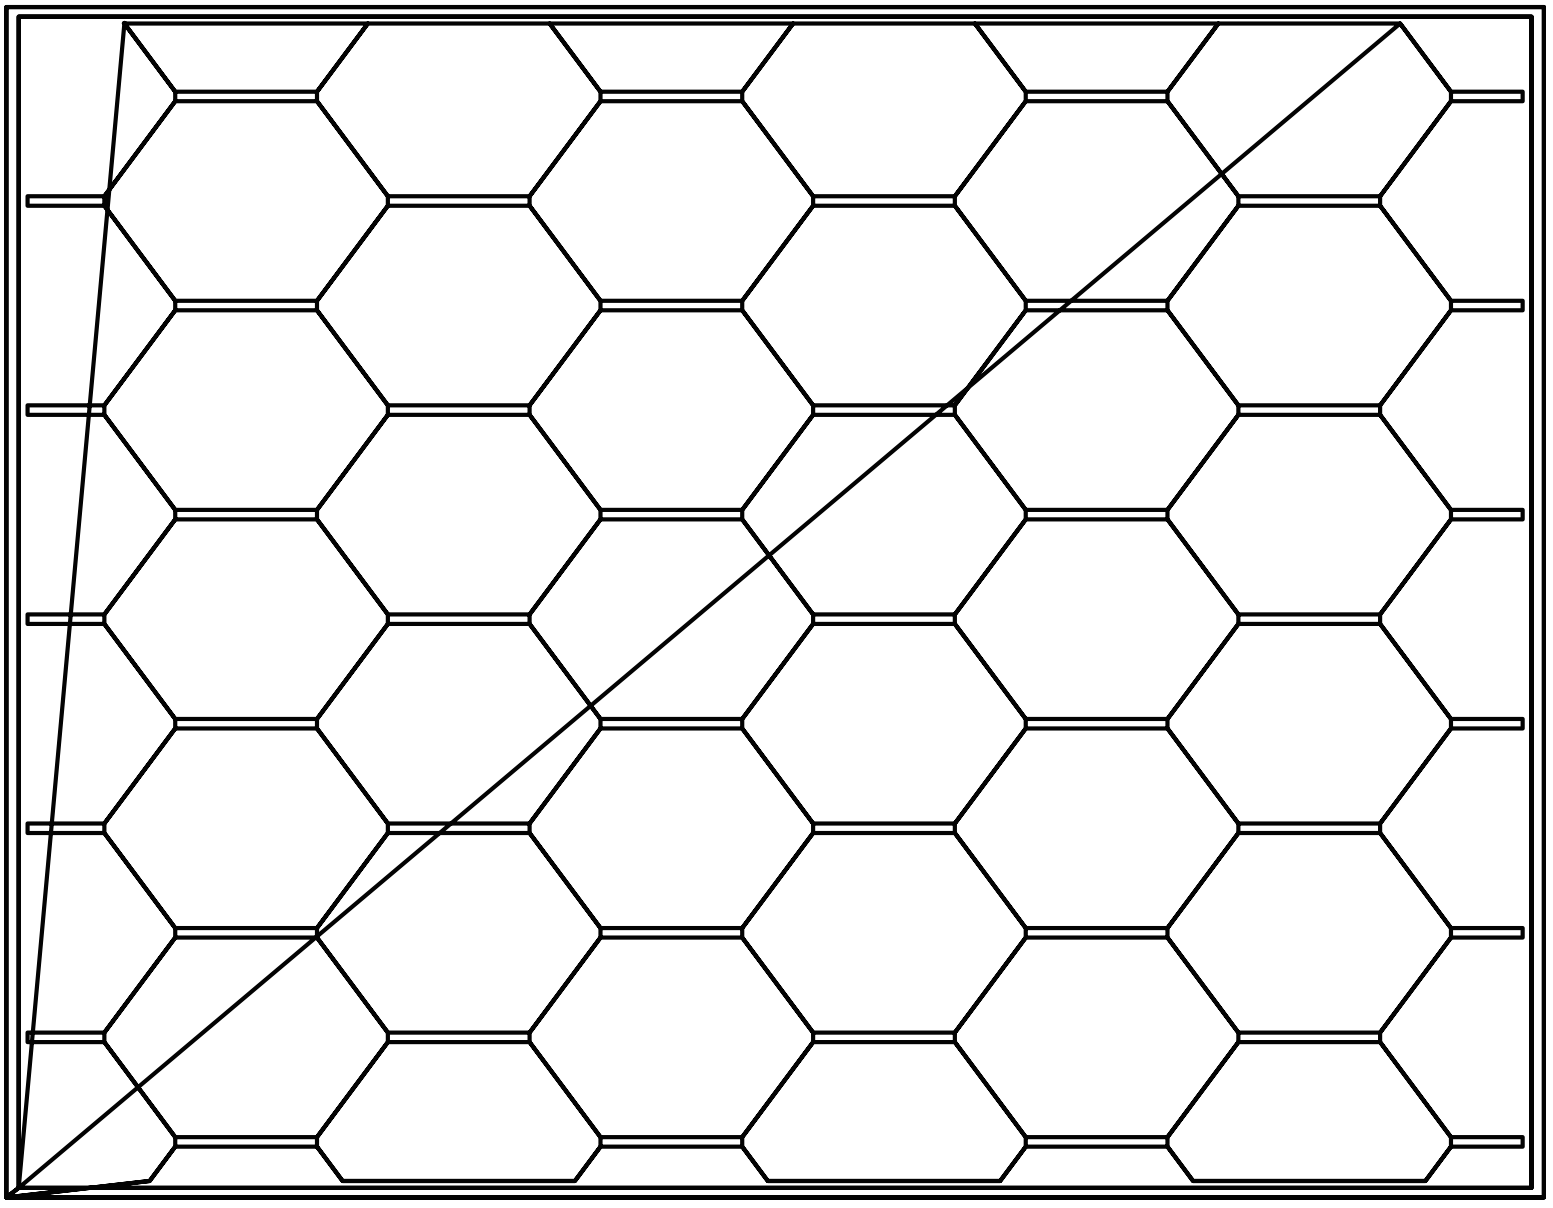
\includegraphics[width=0.18\textwidth]{figs/makerbot_infill_strategy_square_hexagonal.png}
  \label{}
  }
  &
  \subfloat[Moroccan Star]
  {
  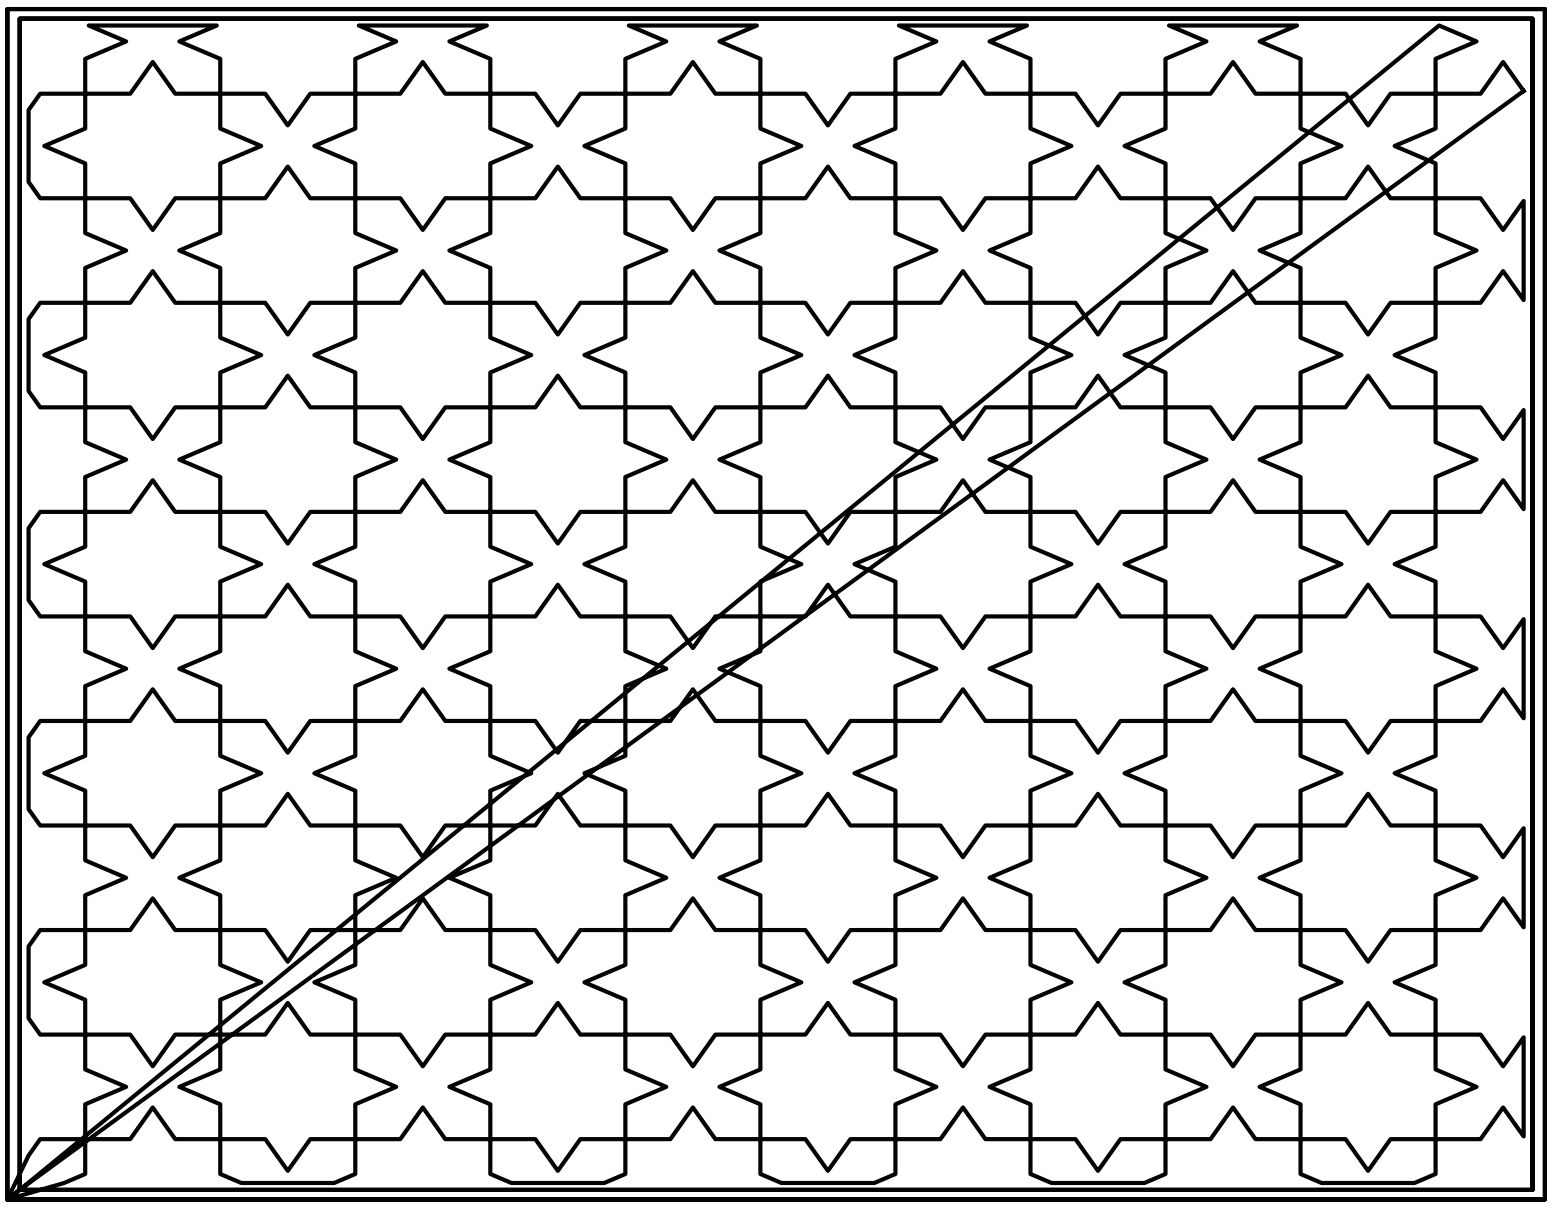
\includegraphics[width=0.18\textwidth]{figs/makerbot_infill_strategy_square_moroccanstar.png}
  \label{}
  }
  &
  \subfloat[Catsfill]
  {
  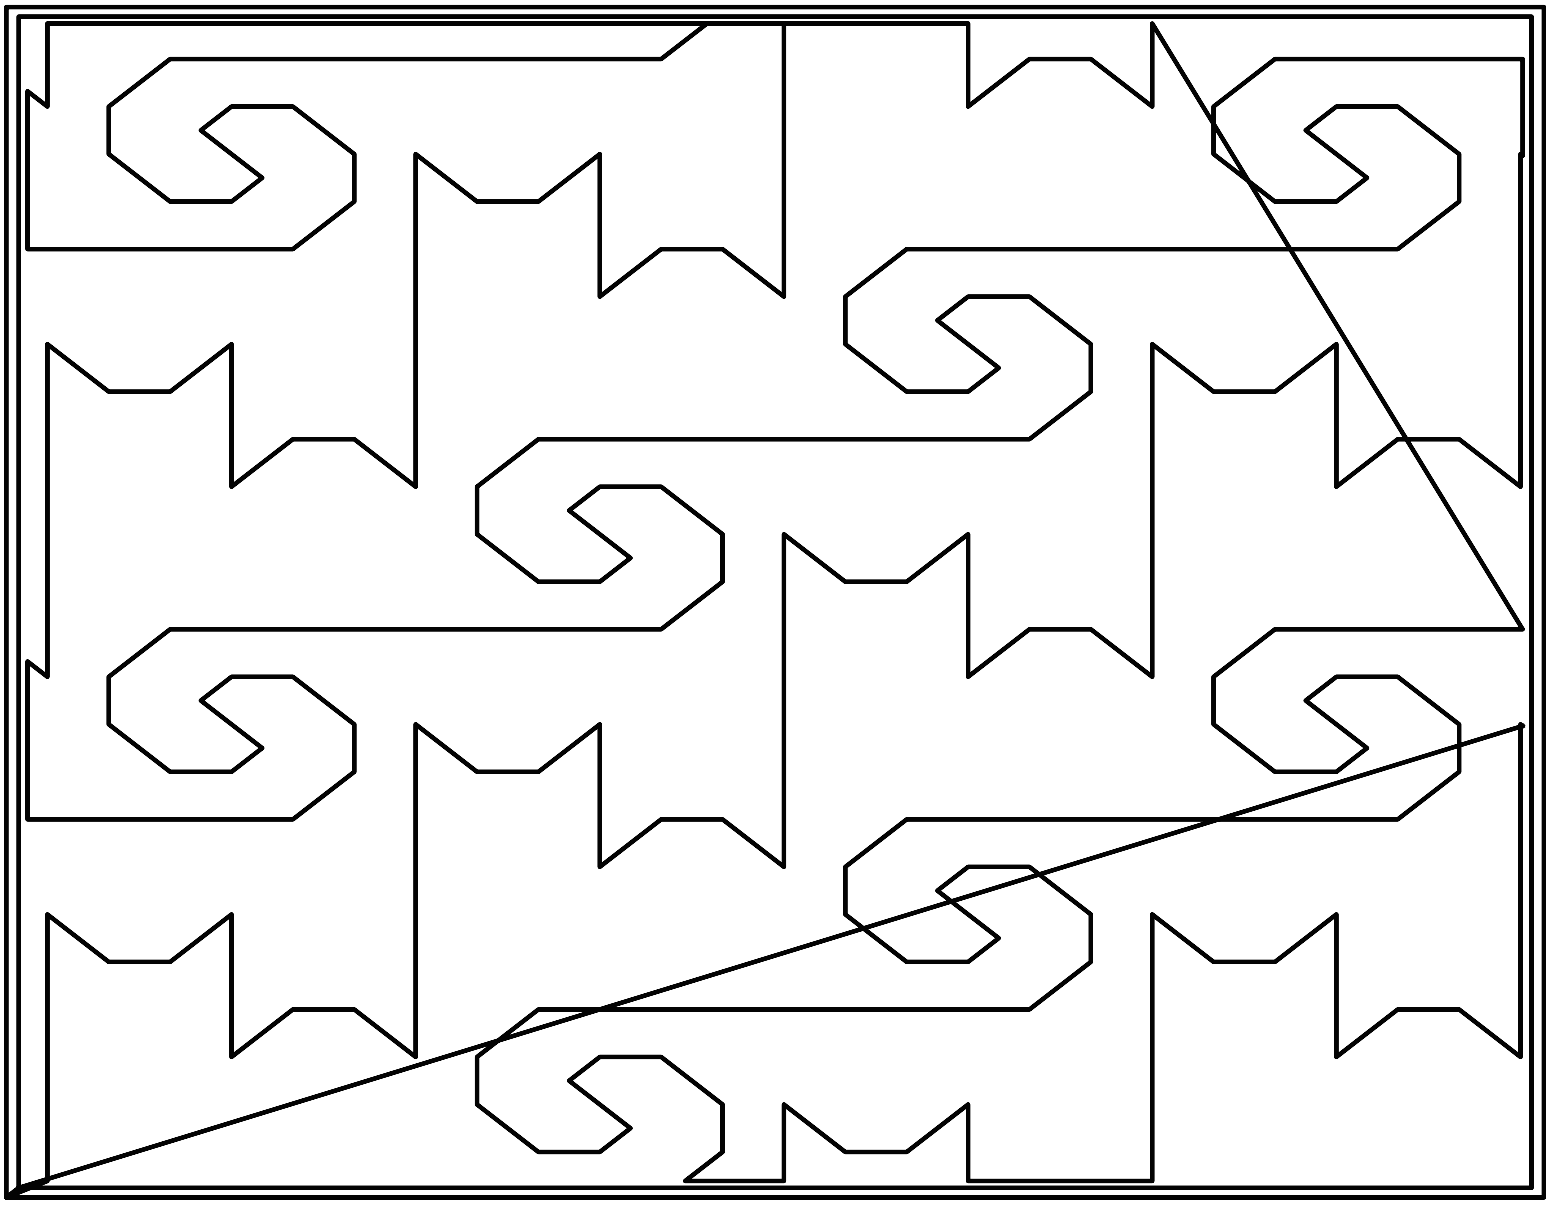
\includegraphics[width=0.18\textwidth]{figs/makerbot_infill_strategy_square_catfill.png}
  \label{}
  }
  &
  \subfloat[Sharkfill]
  {
  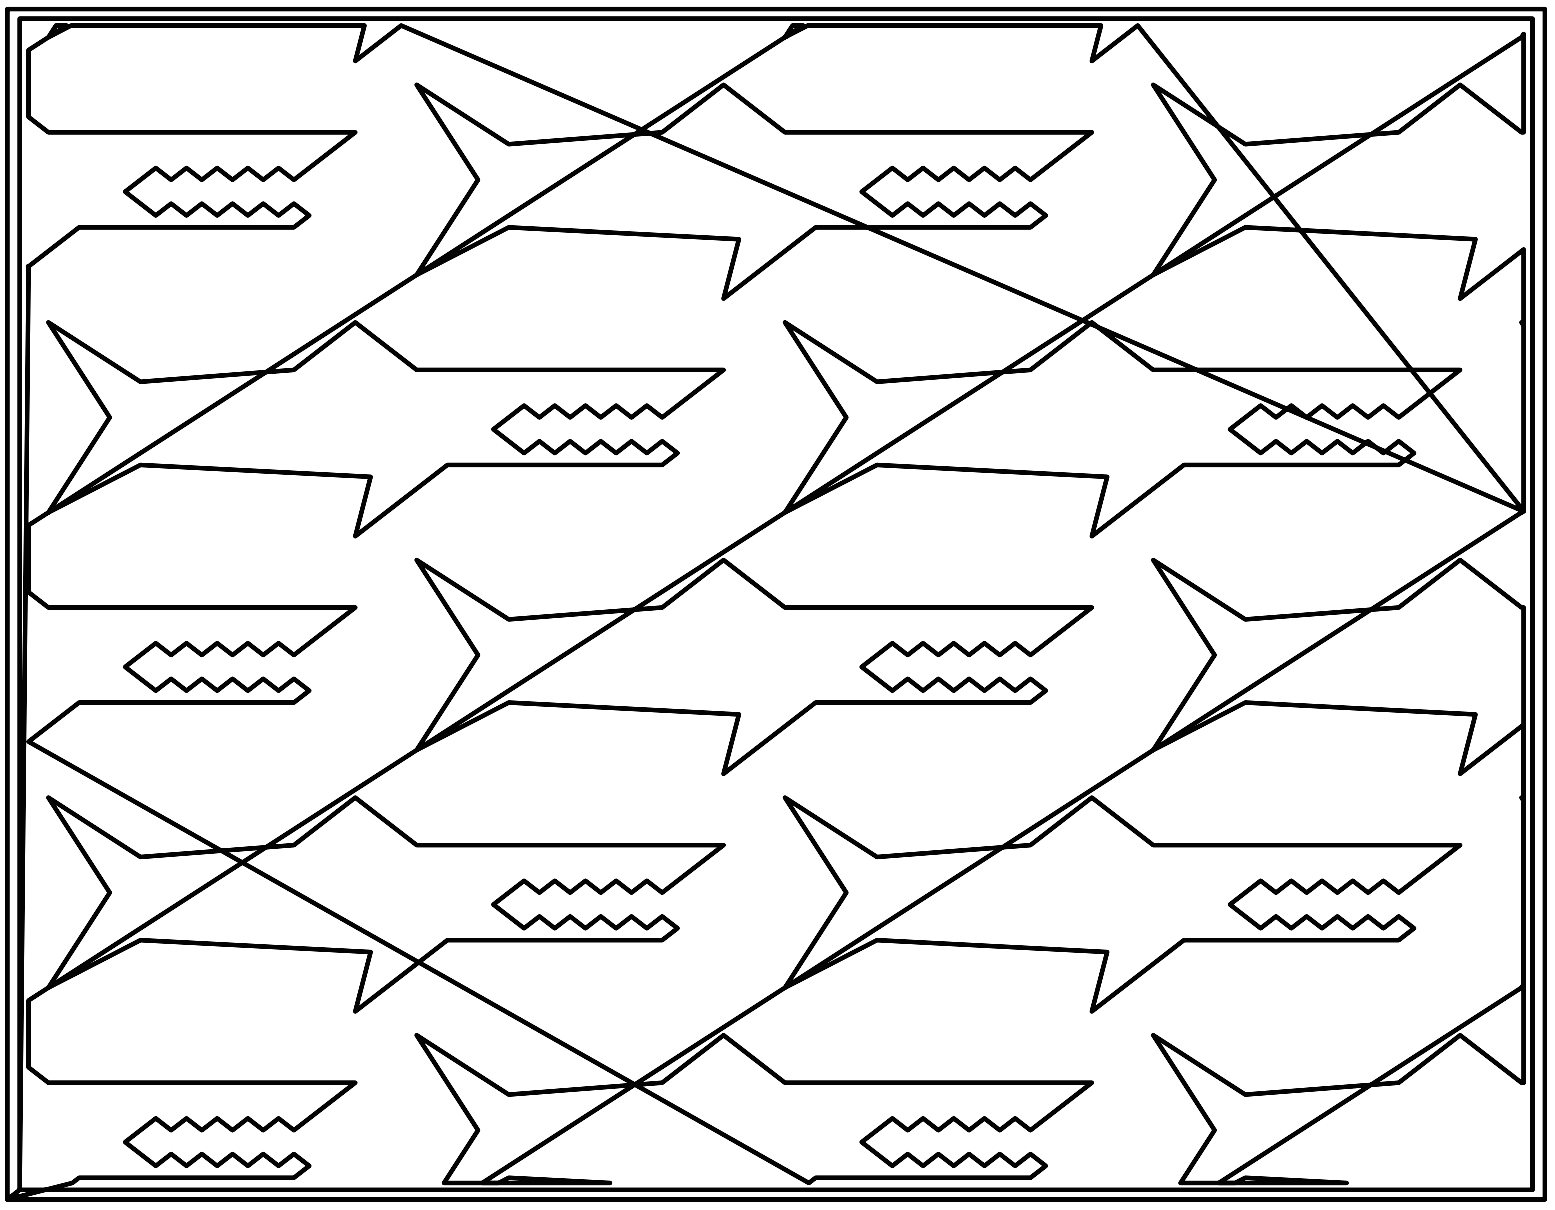
\includegraphics[width=0.18\textwidth]{figs/makerbot_infill_strategy_square_sharkfill.png}
  \label{}
  }
  \\

  \subfloat[Line]
  {
  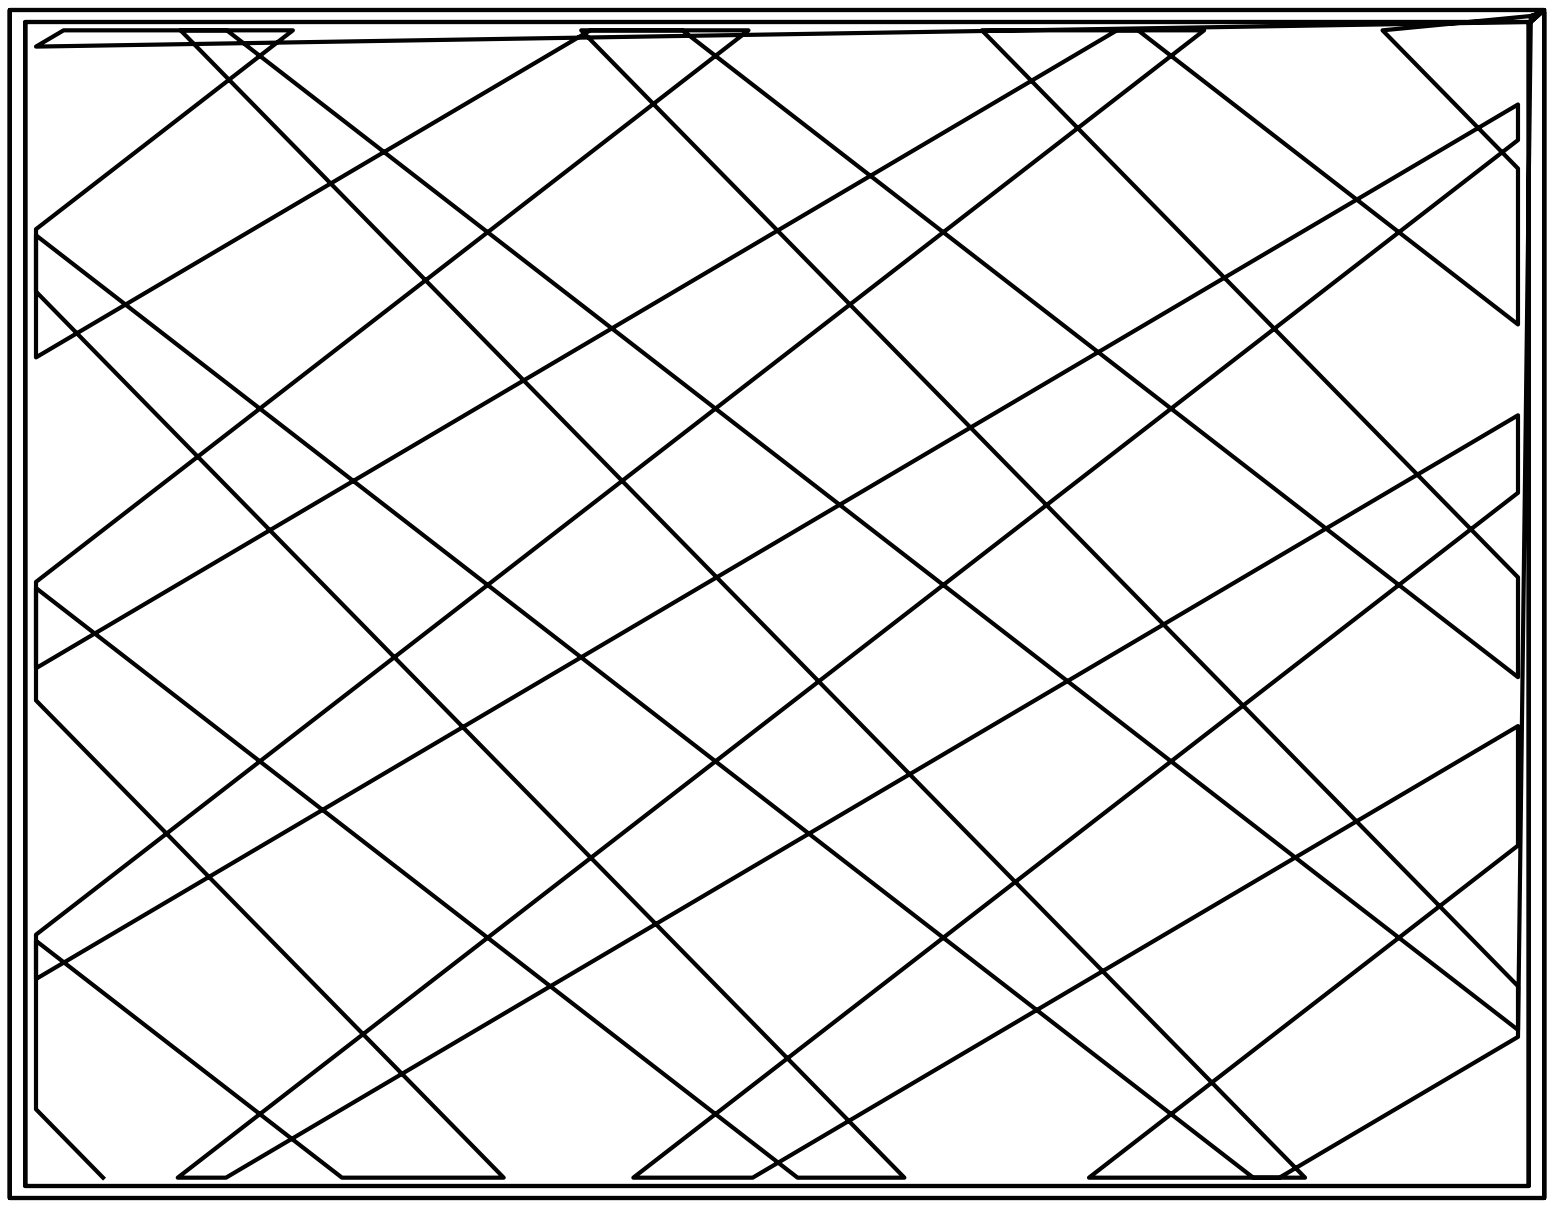
\includegraphics[width=0.18\textwidth]{figs/slic3r_plate_line.png}
  \label{}
  }
  &
  \subfloat[Rectilinear]
  {
  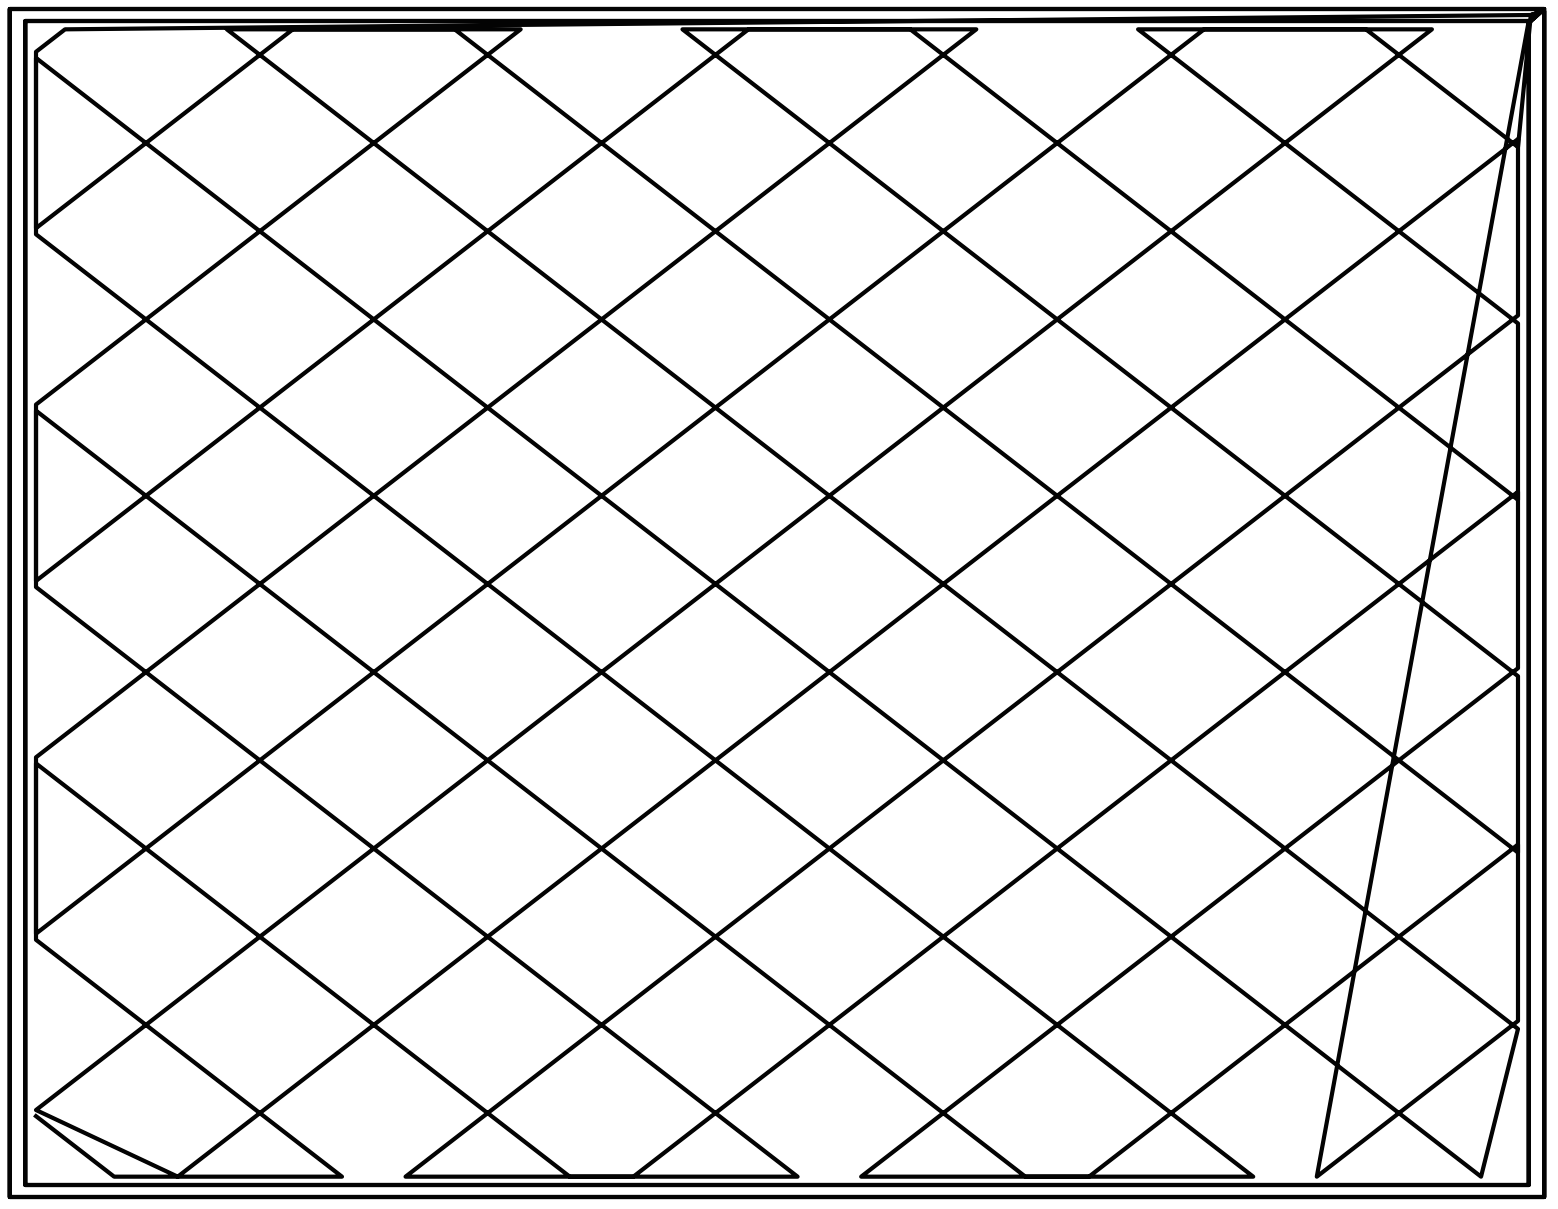
\includegraphics[width=0.18\textwidth]{figs/slic3r_plate_rectilinear.png}
  \label{}
  }
  &
  \subfloat[Concentric]
  {
  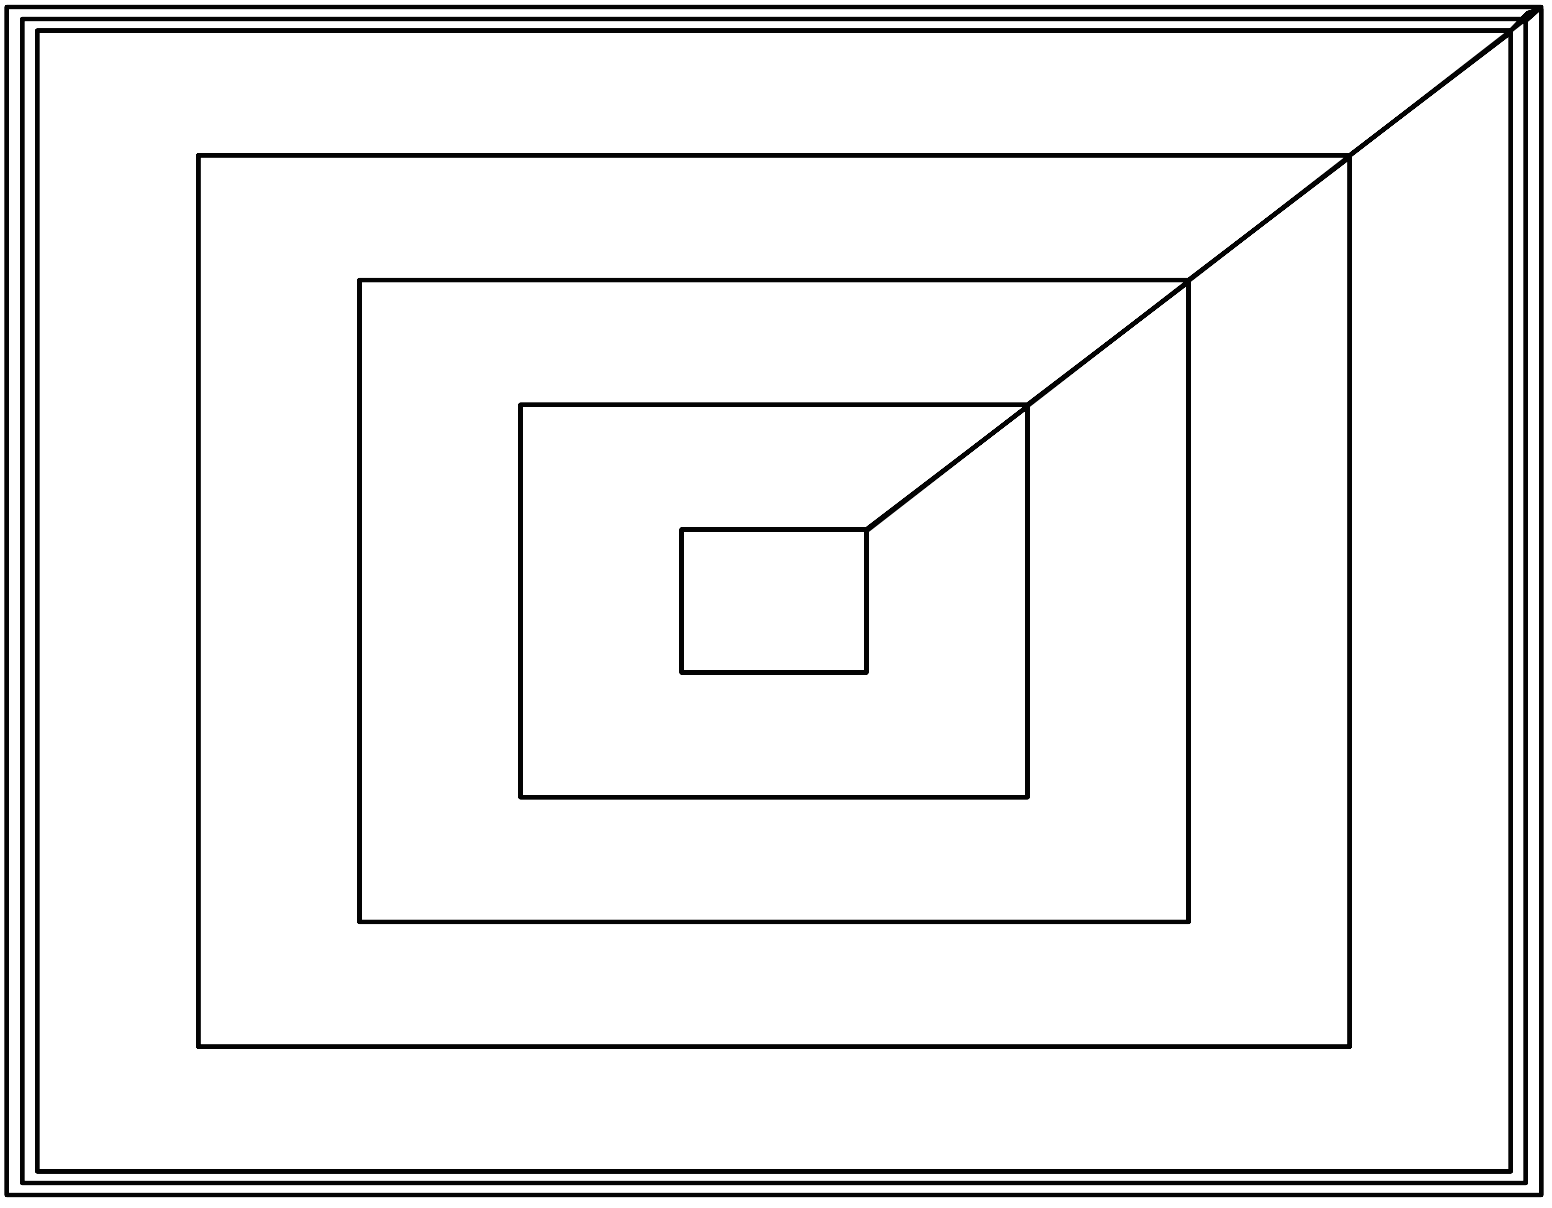
\includegraphics[width=0.18\textwidth]{figs/slic3r_plate_concentric.png}
  \label{}
  }
  &
  \subfloat[Hilbert Curve]
  {
  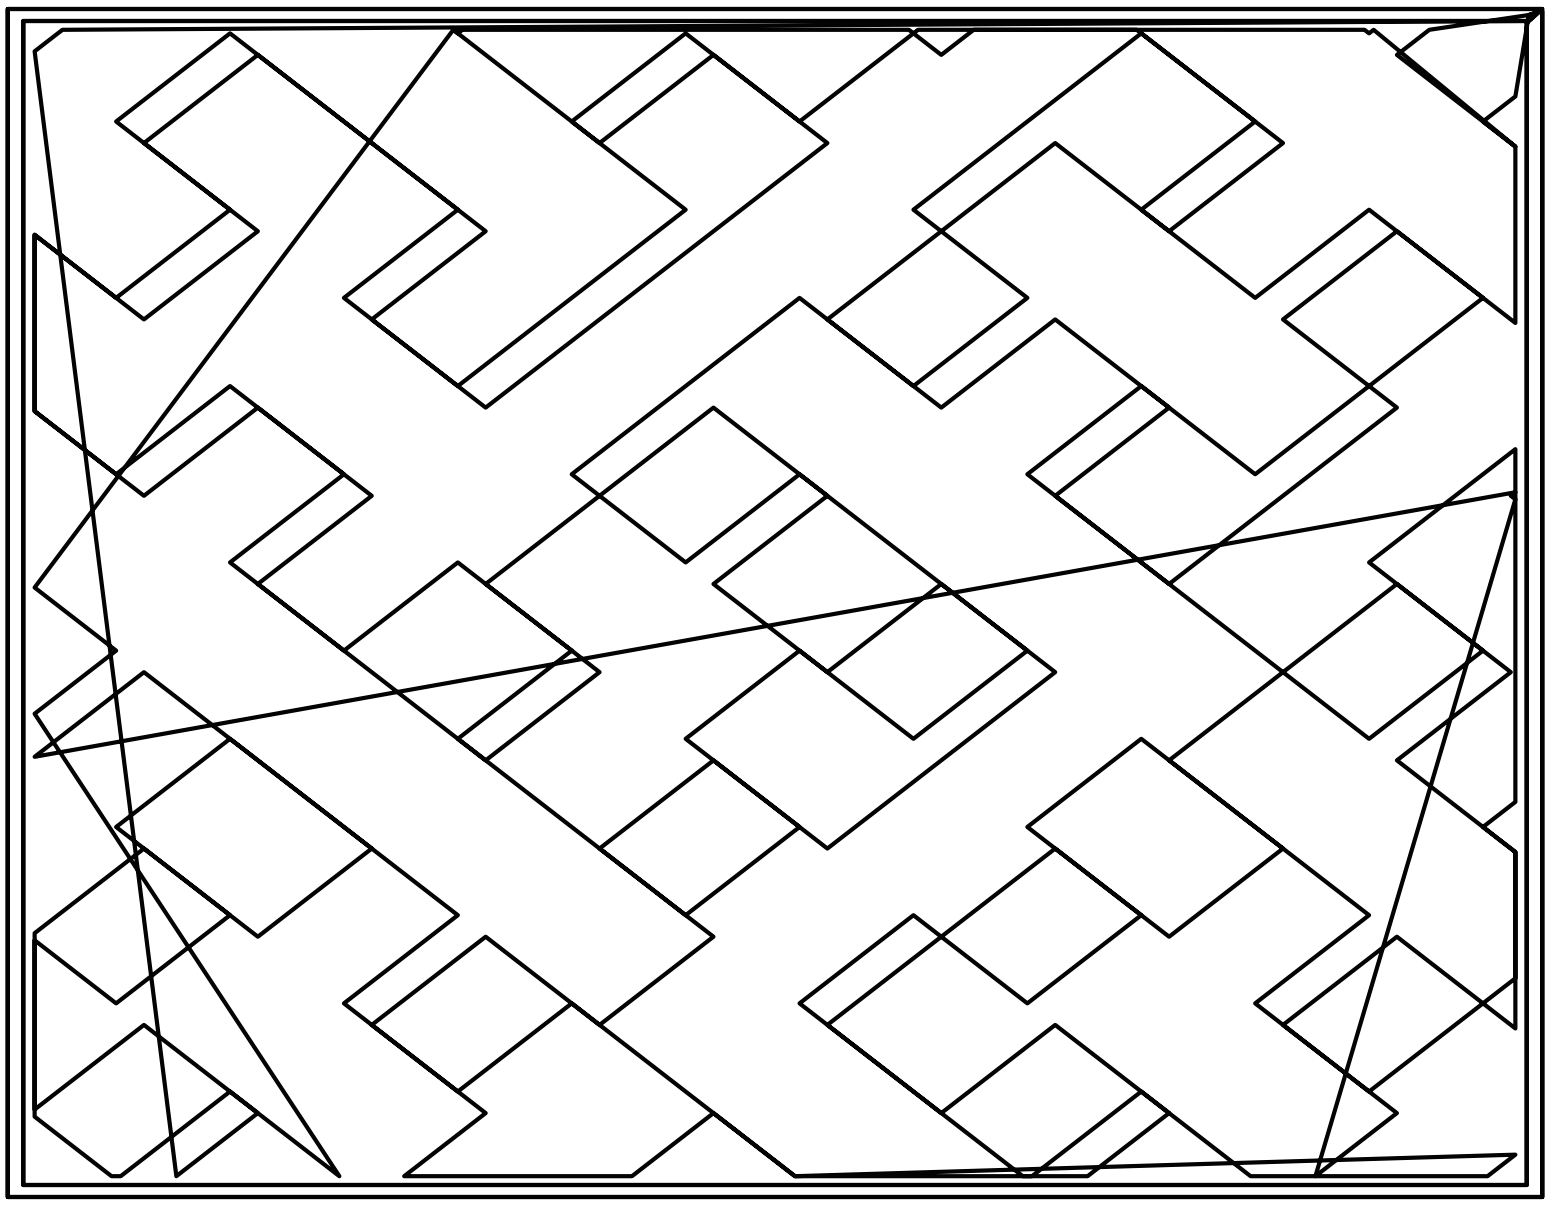
\includegraphics[width=0.18\textwidth]{figs/slic3r_plate_hilbertcurve.png}
  \label{}
  }
  &
  \subfloat[Archimedean Chords]
  {
  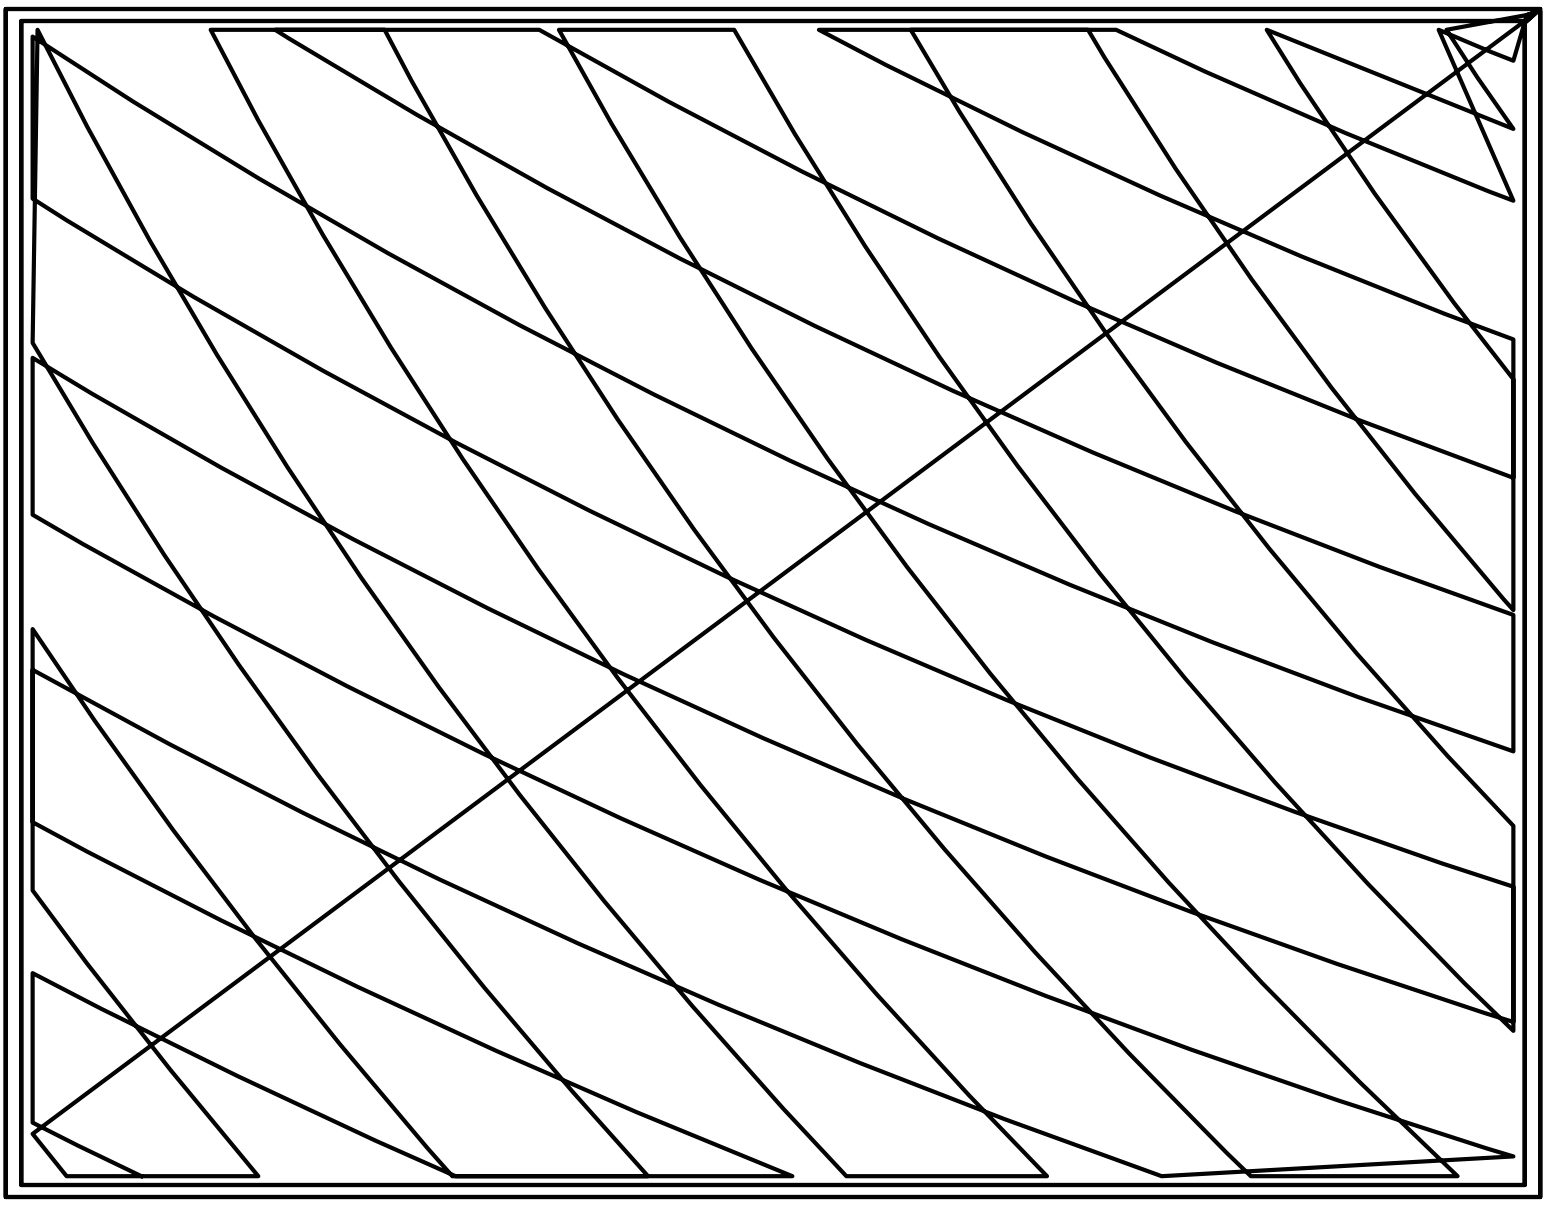
\includegraphics[width=0.18\textwidth]{figs/slic3r_plate_archimedeanchords.png}
  \label{}
  }
  \\

  \end{tabular}
  \vspace{1em}
  \caption{Infill Strategies from MakerWare (a-e) \& Slic3r (f-j) Software}
\label{fig-infills}
\end{figure*}

Rafts\marginnote{Rafts} are printed onto the print bed ahead of the part being printed. This provides an adhesive layer for the part to be printed on and reduces the chance of the print warping and/or separation from the print bed occurring.

Supports\marginnote{Supports} can be selected to help with parts that contain overhangs or features that require bridging. This enables more complex geometries to be produced but at the cost of additional post-processing and finishing of parts.

The level of support can be reduced considerably if you try different orientations of a part on the print bed. In addition, new multi-head printers allow for the printing of soluble support material, which can be dissolved by placing the printed part in water.

Layer height\marginnote[-2em]{Layer Height} is typically measured in \si{\milli\metre}. The larger the height, the quicker the print and coarser the finish. It is often best to leave this parameter at its default setting. Although, there is research looking into adaptive layer heights where the slicing tool will automatically reduce the layer height when the slicer identifies complex areas of geometry.\cite[-6em]{pandey2003}\cite[-1em]{sabourin1996}

The\marginnote{G-Code} language used to communicate motor movements and deposition of the filament.


\subsubsection{Slicing Process} 

Slicing is the process of generating the GCode for a 3D Model. In this section, we will go through the process of slicing a simple rectangular block where we do not have to consider the addition of rafts and supports. Although you will be using a slicing program to automatically do this, it is good to know what is going one behind the scenes. You never know when you may want to generate your own custom GCode for a 3D printer to use. The main steps are:

\begin{enumerate}
  \item Identifying the perimeter geometry
  \item Creating shells
  \item Creating the internal linear mesh
  \item Determining the printer travel path
  \item Creating the GCode printer file
\end{enumerate}

\begin{figure}[h!]
  \centering
  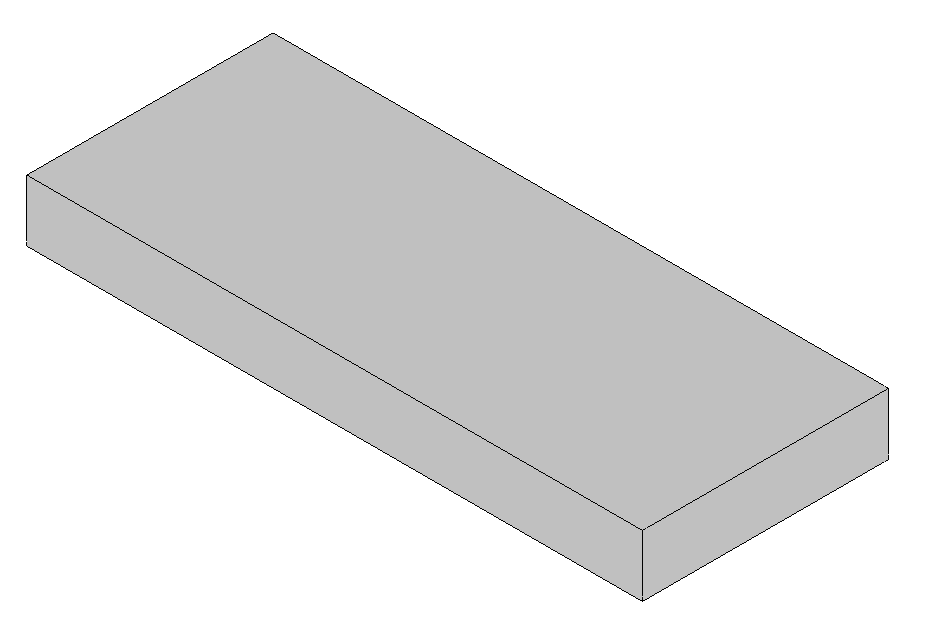
\includegraphics[width=0.7\textwidth]{figs/beam_stl.png}
  \caption{Rectangular block to be sliced}\label{fig-block}
\end{figure}


We\marginnote{Perimeter Identification} will now go through the procedure for one slice of the rectangular block (\cref{fig-block}). The first step is to identify for the perimeter on the plane at which we wish to slice. To achieve this, a slicing plane is generated and the intersections between the plane and the \ac{STL} model are identified (\cref{fig-intersection}). A set of lines is then generated from where the plane intersects the individual polygons of the \ac{STL} file. It is then the case of identifying the connecting path between the lines. This is achieved by taking a single line and identifying the neighbouring line by finding the end points that match. The process then continues to the end of the next line and repeats until the sequences of lines returns to the starting line. This forms a perimeter polygon for the part. There is then a check to see whether any lines remain that do not form part of the chain. If so, a new chain is generated with the remaining lines. This cycle repeats until all the lines are associated to a chain. This enables the identification of complex geometry with multiple perimeters such as a part containing holes and/or cut-outs.

\begin{figure}[h!]
  \center
  \tdplotsetmaincoords{45}{135}
  \begin{tikzpicture}[scale=0.5, tdplot_main_coords]
    \coordinate (O) at (0,0,0);
    \draw[thick] (0, 0, 0) -- (0, 10, 0) -- (4, 10, 0) -- (4, 0, 0) -- (0, 0, 0);
    \draw[thick] (0, 0, 2) -- (0, 10, 2) -- (4, 10, 2) -- (4, 0, 2) -- (0, 0, 2);

    \draw[thick] (0,0,0) -- (0,0,2);
    \draw[thick] (0,10,0) -- (0,10,2);
    \draw[thick] (4,10,0) -- (4,10,2);
    \draw[thick] (4,0,0) -- (4,0,2);

    \draw[fill=gray, fill opacity=0.2] (-0.5, -0.5, 0.6) -- (-0.5, 10.5, 0.6) -- (4.5, 10.5, 0.6) -- (4.5, -0.5, 0.6) -- (-0.5, -0.5, 0.6);
    \draw[dashed] (0, 0, 0.6) -- (0, 10, 0.6) -- (4, 10, 0.6) -- (4, 0, 0.6) -- (0, 0, 0.6);

    \draw[->] (7,5,0) -- (7,6,0) node[right]{x};
    \draw[->] (7,5,0) -- (6,5,0) node[right]{y};
    \draw[->] (7,5,0) -- (7,5,1) node[anchor=south]{z};

  \end{tikzpicture}
  \caption{Cutting planes through the beam STL}
  \label{fig-intersection}
\end{figure}


With\marginnote{Shells} the perimeter identified, one can perform a transform on the perimeter polygon that has an offset applied to create a duplicate perimeter within a filament width of the previous polygon. The number of times this is performed is determined by the number of shells you wish to have for your model.


\begin{figure}[h!]
  \centering
    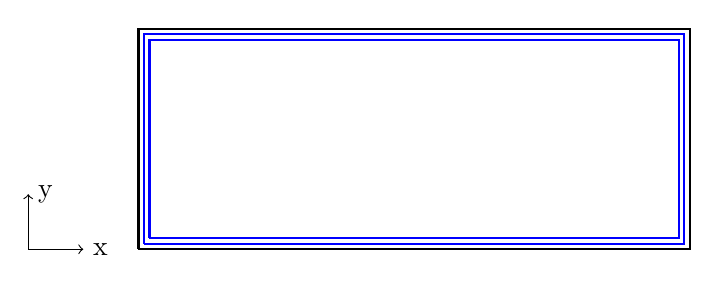
\begin{tikzpicture}[scale=0.7]
      \draw[thick] (0,0) -- (10,0) -- (10,4) -- (0,4) -- (0,0);
      \draw[thick, blue] (0.1,0.1) -- (9.9,0.1) -- (9.9,3.9) -- (0.1,3.9) -- (0.1,0.1);
      \draw[thick, blue] (0.2,0.2) -- (9.8,0.2) -- (9.8,3.8) -- (0.2,3.8) -- (0.2,0.2);
      \draw[->] (-2,0) -- (-1,0) node[right]{x};
      \draw[->] (-2,0) -- (-2,1) node[right]{y};
    \end{tikzpicture}
    \caption{Creating shells from the perimeter polygon}\label{fig-shells}
\end{figure}

The\marginnote{Linear Mesh Generation} third step of the process involves the generation of a set of uniformly distributed vertical and horizontal lines to form the linear infill design for the part. The linear infill width sizing is derived from the infill density perimeter that is set in the software. The process then generates rays along the x \& y axes for the given layer height, and identifies the intersections of rays against the \ac{STL} model of the part (Figures~\ref{fig-shells}a \& \ref{fig-shells}b). For complex geometries, the rays have the potential to intersect the model multiple times and thus, the lines of interest are determined by pairing intersecting points as the ray passes through the model (i.e. points 1 and 2 will form a path and the same goes for 3-4, 5-6, etc\ldots).

\begin{figure*}[h!]
    \centering
    \begin{tabular}{c c}
      \subfloat[Infill ray casting]{
        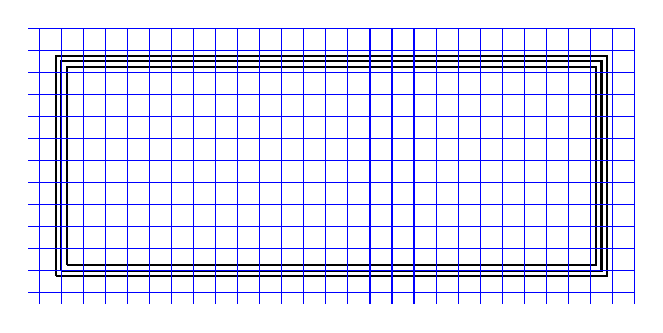
\begin{tikzpicture}[scale=0.7]
        \draw[thick] (0,0) -- (10,0) -- (10,4) -- (0,4) -- (0,0);
        \draw[thick] (0.1,0.1) -- (9.9,0.1) -- (9.9,3.9) -- (0.1,3.9) -- (0.1,0.1);
        \draw[thick] (0.2,0.2) -- (9.8,0.2) -- (9.8,3.8) -- (0.2,3.8) -- (0.2,0.2);
        
        \foreach \y in {-0.3, 0.1, 0.5, ..., 4.5}
          \draw[blue] (-0.5,\y) -- (10.5,\y);
        \foreach \x in {-0.3, 0.1, 0.5, ..., 10.5}
          \draw[blue] (\x,-0.5) -- (\x,4.5);

        %\draw[->] (0,5) -- (1,5) node[right]{x};
        %\draw[->] (0,5) -- (0,6) node[right]{y};
      \end{tikzpicture}
      } &
      \subfloat[Linear Mesh]{
        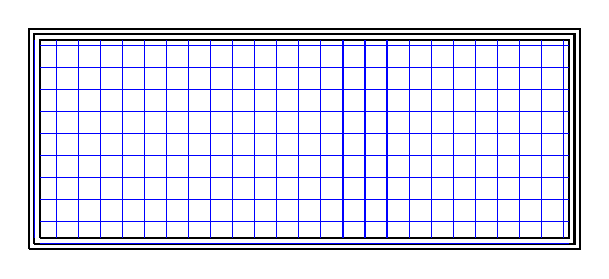
\begin{tikzpicture}[scale=0.7]
        \draw[thick] (0,0) -- (10,0) -- (10,4) -- (0,4) -- (0,0);
        \draw[thick] (0.1,0.1) -- (9.9,0.1) -- (9.9,3.9) -- (0.1,3.9) -- (0.1,0.1);
        \draw[thick] (0.2,0.2) -- (9.8,0.2) -- (9.8,3.8) -- (0.2,3.8) -- (0.2,0.2);
        \foreach \y in {0.1, 0.5, ..., 4}
          \draw[blue] (0.2,\y) -- (9.8,\y);
        \foreach \x in {0.1, 0.5, ..., 10}
          \draw[blue] (\x,0.2) -- (\x,3.8);
      \end{tikzpicture}
      }
    \end{tabular}
    \vspace{1em}
    \caption{Creating shells from the perimeter polygon}\label{fig-shells}
\end{figure*}


With\marginnote[1em]{Printer Travel Path} all the deposition lines defined for the slice, Step 4 creates the path the printer will take to deposit the filament. The printer starts with the outer perimeter path and followed by the inner parameter paths. The process then takes the linear infill lines and increments back and forth for both the horizontal and vertical lines of the mesh so that the travel of the printer head between depositions is minimised.

\begin{figure}[h!]
  \centering
    \begin{tikzpicture}[scale=1, decoration={markings,mark=at position 0.5 with {\arrow{>}}}]
      \draw[thick,postaction={decorate},->] (0,0) -- (10,0); 
      \draw[thick,postaction={decorate},->] (10,0) -- (10,4); 
      \draw[thick,postaction={decorate},->] (10,4) -- (0,4); 
      \draw[thick,postaction={decorate},->] (0,4) -- (0,0); 

      \draw[thick,postaction={decorate},->] (0.1,0.1) -- (9.9,0.1); 
      \draw[thick,postaction={decorate},->] (9.9,0.1) -- (9.9,3.9); 
      \draw[thick,postaction={decorate},->] (9.9,3.9) -- (0.1,3.9); 
      \draw[thick,postaction={decorate},->] (0.1,3.9) -- (0.1,0.1);

      \draw[thick,postaction={decorate},->] (0.2,0.2) -- (9.8,0.2); 
      \draw[thick,postaction={decorate},->] (9.8,0.2) -- (9.8,3.8); 
      \draw[thick,postaction={decorate},->] (9.8,3.8) -- (0.2,3.8); 
      \draw[thick,postaction={decorate},->] (0.2,3.8) -- (0.2,0.2);

      \foreach \y in {1.0, 2.0, 3.0, 4}
        \draw[thick,blue,postaction={decorate},->] (9.8,\y) --(0.2,\y);

      \foreach \y in {0.5, 1.5, 2.5, 3.5}
        \draw[thick,blue,postaction={decorate},->] (0.2,\y) -- (9.8,\y);
        
      \foreach \x in {0.5, 1.5, 2.5, 3.5, 4.5, 5.5, 6.5, 7.5, 8.5, 9.5}
        \draw[thick,blue,postaction={decorate},->]  (\x,3.8) -- (\x,0.2);

      \foreach \x in {1, 2, 3, 4, 5, 6, 7, 8, 9, 10}
        \draw[thick,blue,postaction={decorate},->] (\x,0.2) -- (\x,3.8);

      \draw[thick,red,->] (0,0) -- (0.1,0.1);
      \draw[thick,red,->] (0.1,0.1) -- (0.2,0.2);

      \draw[thick,red,->] (0.2,0.2) -- (0.2,0.5); 
      \draw[thick,red,->] (0.2,1.0) -- (0.2,1.5);
      \draw[thick,red,->] (0.2,2.0) -- (0.2,2.5);
      \draw[thick,red,->] (0.2,3.0) -- (0.2,3.5);

      \draw[thick,red,->] (9.8,0.5) -- (9.8,1.0); 
      \draw[thick,red,->] (9.8,1.5) -- (9.8,2.0);
      \draw[thick,red,->] (9.8,2.5) -- (9.8,3.0);

      \draw[thick,red,->] (9.8,3.5) -- (9.5,3.8); % top right diagonal

      \draw[very thick,black] (0,4.4) -- (0.2,4.4) node[pos=1.0,anchor=west] {Shell Line};
      \draw[very thick,blue] (3,4.4) -- (3.2,4.4) node[pos=1.0,anchor=west,black] {Infill Line};
      \draw[very thick,red] (6,4.4) -- (6.2,4.4) node[pos=1.0,anchor=west,black] {Travel Line};

      % [To Finish]
    \end{tikzpicture}
    \caption{Generated printer path}\label{fig-printer-path}
\end{figure}

Stage 5\marginnote{G-Code} then generates the GCode file containing the printer head movements. Before the commands are placed in the GCode, there is a pre-amble section that provides the initial settings and parameters for the printer. The co-ordinates are then translated into GCode commands that contain both the co-ordinates and feed rates for the printer filament. A post-amble is then appended to the document, which tells the printer to return to its initial state and cool down.


\subsubsection{Strengths}

One\marginnote{Convenience} of the main strengths of 3D printing is its convenience. The parts are typically a fraction of the cost compared to other prototyping methods and the process if very quick. Parts are often printed in hours enabling you to view and amend models quickly, making the design process more fluid. The process is also very simple and easy to use requiring little knowledge to get up and running. 

3D\marginnote{Structure} Printing is also incredibly flexible in the geometry that it can print and is good for small, unusual and awkwardly shaped components. It is also very good for free-form surfaces and is often used in producing casings for products. It also has a limited capability to produce some functional items including screw threads, dowels and holes, spacers and the material can also be tapped.

\subsubsection{Weaknesses}

However\marginnote{Quality and Finish}, 3D Printing is not the answer to all of your prototyping and manufacturing needs. 3D Printers still find it a challenge with features that require high tolerances. In particular, cylindricity, parallel and perpendicularity is often challenging due to the nature of printing in layers and the level of accuracy the printers can attain with the stepper motors. 

Surface quality is generally good for prototypes but post-processing is required for a truly smooth surface. Small bumps and deviations can appear on the surface as the filament cools. In addition, there is a lack of consistency in the print quality and accuracy for the same print instructions.


\subsubsection{Guidelines}

Always\marginnote{Evaluate Different Orientations} double check whether the model has been placed in its optimum position for printing. Re-orienting the model within the slicing software can significantly reduce number of supports that may be required.

Even-though\marginnote{Avoid Overhangs} 3D printing can deal with overhangs by using supports, significant reductions in manufacturing time can be achieved by generating geometry that does not require the use of supports. This reduces manufacturing time as supports do not need to be printed, a reduction in material use and post-processing time owing to the need to remove them from the structure.

The\marginnote{Keep to Low Infill Densities} process is also less suitable for large parts and parts, which require 100\% infill. This is due to the time it takes and the greater likelihood of the print failing due to printer operating for a long time.

Although\marginnote{Place Prints near the Centre of the Bed} the printers are regularly calibrated, it is still good practice to place the component near the centre of the bed. And even-though the printers can handle the printing of multiple parts at once, this introduces issues in the filament maintaining adhesion between layers as the component will cool whilst the printer head is busy on a different component.